\documentclass[a4paper]{article}

\def\nbook {Introduction to Quantum Mechanics \\ Second Edition}
\def\nbookshort {Griffiths Quantum Mechanics}

% Shared preamble. The fallback lets the document build whether the working
% directory is its own folder or the project root.
\IfFileExists{headerintroquantummechanics.tex}{%%%%%%%%%%%%%%%%%%%%
% AUTHOR AND HEADER
% define \nbook
%%%%%%%%%%%%%%%%%%%%

\makeatletter
\ifx \nauthor\undefined
	\def\nauthor{David A. Lee}
\else
\fi

\author{\nbook \\ \small David J. Griffiths \\ \small Solutions by \nauthor}
\date{}

%%%%%%%%%%%%%%%%%%%%
% PACKAGES
%%%%%%%%%%%%%%%%%%%%

\usepackage{alltt} 
\usepackage{amsfonts}
\usepackage{amsmath}
\usepackage{amssymb}
\usepackage{amsthm}
\usepackage{bm}
\usepackage{booktabs}
\usepackage{braket} % \bra, \ket, \braket; not `physics`, which clashes with \abs/\norm below
\usepackage{caption}
\usepackage{centernot}
\usepackage{enumitem}
\usepackage{fancyhdr}
\usepackage[T1]{fontenc}
\usepackage{graphicx}
% The documents sit one level below the project root, where the chapN/ figure
% folders live. Listing both "./" and "../"
% lets those be referenced the same way regardless of where the build runs.
\graphicspath{{./}{../}}
\usepackage{mathdots}
\usepackage{mathtools}
% \usepackage{microtype}
\usepackage{multirow}
\usepackage{pdflscape}
\usepackage{pgfplots}
\pgfplotsset{compat=1.18}
\usepackage{siunitx}
\usepackage{slashed}
\usepackage{tabularx}
\usepackage{tikz}
\usepackage{titletoc}
\usepackage{tkz-euclide}
\usepackage[normalem]{ulem}
\usepackage{url}
\usepackage[all]{xy}
\usepackage{imakeidx}

% fonts
% use \textsf for the sans family (problem titles, section headings)
% Latin Modern Sans, not CM Bright: cmbr under T1 has no Type 1 outlines, so it
% renders as Type 3 bitmaps, which TeXpresso's viewer cannot draw at all.
\renewcommand{\sfdefault}{lmss} % keeps default font Computer Modern Roman

% makeindex for table of contents
\makeindex[intoc, title=Index]
\indexsetup{othercode={\lhead{ Index }}}

% table of contents remove numbering
\usepackage{tocloft} % for coloring subsections -- note that sections have standard document hyperlink coloring, i.e. color = doc
\setcounter{secnumdepth}{0} % remove numbering
\renewcommand{\cftsubsecfont}{\hypersetup{linkcolor=subsect!90}} % subsection coloring
\renewcommand{\cftsubsubsecfont}{\hypersetup{linkcolor=subsubsect!90}} % subsubsection coloring
\renewcommand{\contentsname}{\textsf{Table of Contents}}

% pagestyle
\pagestyle{fancyplain}

% header
\lhead{	\nouppercase{\leftmark} }
\ifx \nextra \undefined
  \rhead{
    \ifnum\thepage=1
    \else
      \nbookshort \  | \nauthor
    \fi}
\else
  \rhead{
    \ifnum\thepage=1
    \else
      \nbookshort (\nextra)
    \fi}
\fi

% proof environment
\newcommand{\prooffont}{\scshape}
\usepackage{xpatch}
\tracingpatches
\xpatchcmd{\proof}{\itshape}{\prooffont}{}{}

% Python environment (for typesetting Python code)

% Default fixed font does not support bold face
\DeclareFixedFont{\ttb}{T1}{txtt}{bx}{n}{8} % for bold
\DeclareFixedFont{\ttm}{T1}{txtt}{m}{n}{8}  % for normal

% Custom colors
\usepackage{color}
\definecolor{deepblue}{rgb}{0,0,0.5}
\definecolor{deepred}{rgb}{0.6,0,0}
\definecolor{deepgreen}{rgb}{0,0.5,0}

\usepackage{listings}

% Python style for highlighting
\newcommand\pythonstyle{\lstset{
language=Python,
basicstyle=\ttm,
morekeywords={self},              % Add keywords here
keywordstyle=\ttb\color{deepblue},
emph={MyClass,__init__},          % Custom highlighting
emphstyle=\ttb\color{deepred},    % Custom highlighting style
stringstyle=\color{deepgreen},
frame=tb,                         % Any extra options here
showstringspaces=false
}}


% Python environment
\lstnewenvironment{python}[1][]
{
\pythonstyle
\lstset{#1}
}
{}

% Python for external files
\newcommand\pythonexternal[2][]{{
\pythonstyle
\lstinputlisting[#1]{#2}}}

% Python for inline
\newcommand\pythoninline[1]{{\pythonstyle\lstinline!#1!}}

%%%%%%%%%%%%%
% FUNCTIONS %
%%%%%%%%%%%%%

\DeclarePairedDelimiter\abs{\lvert}{\rvert}%
% plain \abs{x} autosizes like \left| x \right|; \abs*{x} keeps fixed-size bars
\DeclarePairedDelimiter\absfixed{\lvert}{\rvert}%
\RenewDocumentCommand{\abs}{s}{\IfBooleanTF{#1}{\absfixed}{\absfixed*}}%
\DeclarePairedDelimiter\norm{\lVert}{\rVert}%
% plain \bra, \ket, \braket autosize like braket's \Bra, \Ket, \Braket (including
% the | separators); starred forms keep braket's fixed-size delimiters
\let\brafixed\bra
\let\ketfixed\ket
\let\braketfixed\braket
\RenewDocumentCommand{\bra}{s m}{\IfBooleanTF{#1}{\brafixed{#2}}{\Bra{#2}}}%
\RenewDocumentCommand{\ket}{s m}{\IfBooleanTF{#1}{\ketfixed{#2}}{\Ket{#2}}}%
\RenewDocumentCommand{\braket}{s m}{\IfBooleanTF{#1}{\braketfixed{#2}}{\Braket{#2}}}%

%%%%%%%%%%%%%%%%%%%%
% DOCUMENT GEOMETRY
%%%%%%%%%%%%%%%%%%%%

\ifx \ntrim \undefined
\else
  \usepackage{geometry}
  \geometry{
	  papersize={379pt, 699pt},
	  textwidth=345pt,
	  left=17pt,
	  top=54pt,
	  right=17pt,
  }
\fi

% maketitle statement
\title{}
\ifx \nisofficial \undefined
\let\@real@maketitle\maketitle
\renewcommand{\maketitle}{\@real@maketitle\begin{center}\begin{minipage}[c]{0.9\textwidth}\centering\footnotesize All errors, typographical and substantive, and other offenses, are entirely my own.\end{minipage}\end{center}}
\else
\fi

%%%%%%%%%%%%%%%%%%%%
% THEOREMS
%%%%%%%%%%%%%%%%%%%%

%\theoremstyle{definition}
\newtheorem*{axiom}{Axiom}
\newtheorem*{claim}{Claim}
\newtheorem*{conjecture}{Conjecture}
\newtheorem*{cor}{Corollary}
%\newtheorem*{dfn}{Definition}
\newtheorem*{eg}{Example}
\newtheorem*{ex}{Exercise}
%\newtheorem*{lemma}{Lemma}
\newtheorem*{prop}{Proposition}
%\newtheorem*{thm}{Theorem}
\newtheorem*{remark}{Remark}
\newtheorem*{warning}{Warning}

%%%%%%%%%%%%%%%%%%%%
% FORMATTING AESTHETICS
%%%%%%%%%%%%%%%%%%%%

% itemize bullets
\renewcommand{\labelitemi}{-}
\renewcommand{\labelitemii}{$\circ$}
\renewcommand{\labelenumi}{(\roman{*})}

% new page section
%\let\stdsection\section
%\renewcommand\section{\newpage\stdsection}

% new page subsection
%\let\stdsubsection\subsection
%\renewcommand\subsection{\newpage\stdsubsection}

%%%%%%%%%%%%%%%%%%%%
% \mathbb commands
%%%%%%%%%%%%%%%%%%%%

\newcommand{\C}{\mathbb{C}}
\newcommand{\N}{\mathbb{N}}
\newcommand{\Q}{\mathbb{Q}}
\newcommand{\R}{\mathbb{R}}
\newcommand{\Z}{\mathbb{Z}}

%%%%%%%%%%%%%%%%%%%%
% Complex Numbers
%%%%%%%%%%%%%%%%%%%%

\DeclareMathOperator{\Real}{Re}
\DeclareMathOperator{\Imag}{Im}

%%%%%%%%%%%%%%%%%%%%
% Optimization
%%%%%%%%%%%%%%%%%%%%

\DeclareMathOperator*{\argmax}{arg\,max}

%%%%%%%%%%%%%%%%%%%%
% Probability Operators
%%%%%%%%%%%%%%%%%%%%

\DeclareMathOperator{\Bernoulli}{Bernoulli}
\DeclareMathOperator{\betaD}{Beta}
\DeclareMathOperator{\bias}{\textsf{bias}}
\DeclareMathOperator{\binomial}{Binomial}
\DeclareMathOperator{\corr}{Corr}
\DeclareMathOperator{\cov}{\textsf{Cov}}
\DeclareMathOperator{\Exp}{Exp}
\DeclareMathOperator{\gammaD}{Gamma}
\DeclareMathOperator{\mse}{\textsf{MSE}}
\DeclareMathOperator{\multinomial}{Multinomial}
\DeclareMathOperator{\Poisson}{Poisson}
\DeclareMathOperator{\sd}{sd}
\DeclareMathOperator{\se}{\textsf{se}}
\DeclareMathOperator{\Uniform}{Uniform}
\newcommand{\Prob}{\mathbb{P}}
\newcommand{\var}{\mathbb{V}}
\newcommand{\E}{\mathbb{E}}

%%%%%%%%%%%%%%%%%%%%
% TCOLORBOX CODE FROM SeniorMars
%%%%%%%%%%%%%%%%%%%%

%\usepackage[varbb]{newpxmath} changes math font to newpxmath
\usepackage{xfrac}
\usepackage[makeroom]{cancel}
\usepackage{mathtools}
\usepackage{bookmark}
\usepackage{enumitem}
\usepackage{hyperref}
\usepackage{theoremref}
\hypersetup{
	pdftitle={Assignment},
	colorlinks=true, linkcolor=doc!90,
	bookmarksnumbered=true,
	bookmarksopen=true
}
\usepackage[most,many,breakable]{tcolorbox}
\usepackage{xcolor}
\usepackage{varwidth}
\usepackage{varwidth}
\usepackage{etoolbox}
%\usepackage{authblk}
\usepackage{nameref}
\usepackage{multicol,array}
\usepackage{tikz-cd}
\usepackage[ruled,vlined,linesnumbered]{algorithm2e}
\usepackage{comment} % enables the use of multi-line comments (\ifx \fi)
\usepackage{import}
\usepackage{xifthen}
\usepackage{pdfpages}
\usepackage{transparent}

\newcommand\mycommfont[1]{\footnotesize\ttfamily\textcolor{blue}{#1}}
\SetCommentSty{mycommfont}
\newcommand{\incfig}[1]{%
    \def\svgwidth{\columnwidth}
    \import{./figures/}{#1.pdf_tex}
}

\usepackage{tikzsymbols}

% colors -- change them as you may!

\definecolor{myg}{RGB}{56, 140, 70}
\definecolor{myb}{RGB}{45, 111, 177}
\definecolor{myr}{RGB}{199, 68, 64}
\definecolor{mytheorembg}{HTML}{F2F2F9}
\definecolor{mytheoremfr}{HTML}{00007B}
\definecolor{mylenmabg}{HTML}{FFFAF8}
\definecolor{mylenmafr}{HTML}{983b0f}
\definecolor{mypropbg}{HTML}{f2fbfc}
\definecolor{mypropfr}{HTML}{191971}
\definecolor{myexamplebg}{HTML}{F2FBF8}
\definecolor{myexamplefr}{HTML}{88D6D1}
\definecolor{myexampleti}{HTML}{2A7F7F}
\definecolor{mydefinitbg}{HTML}{E5E5FF}
\definecolor{mydefinitfr}{HTML}{3F3FA3}
\definecolor{notesgreen}{RGB}{0,162,0}
\definecolor{myp}{RGB}{197, 92, 212}
\definecolor{mygr}{HTML}{880808}
\definecolor{myred}{RGB}{127,0,0}
\definecolor{myyellow}{RGB}{169,121,69}
\definecolor{myexercisebg}{HTML}{F2FBF8}
\definecolor{myexercisefg}{HTML}{88D6D1}
\definecolor{doc}{RGB}{0,0,255}
\definecolor{subsect}{RGB}{255,0,0}
\definecolor{subsubsect}{RGB}{128,0,255}
\definecolor{question}{HTML}{3FB69E}

%================================
% THEOREM BOX
%================================

%\providecommand\theoremnumber{}
\tcbuselibrary{theorems,skins,hooks}
\newtcbtheorem{Theorem}{Theorem}
{%
	enhanced,
	breakable,
	colback = mytheorembg,
	frame hidden,
	boxrule = 0sp,
	borderline west = {2pt}{0pt}{mytheoremfr},
	sharp corners,
	detach title,
	before upper = \tcbtitle\par\smallskip,
	coltitle = mytheoremfr,
	fonttitle = \bfseries\sffamily,
	description font = \mdseries,
	separator sign none,
	segmentation style={solid, mytheoremfr},
}
{th}


%================================
% Question BOX
%================================

\makeatletter
\newtcbtheorem{question}{Problem}{enhanced,
	breakable,
	colback=white,
	colframe=question,
	attach boxed title to top left={yshift*=-\tcboxedtitleheight},
	fonttitle=\bfseries\sffamily,
	title={#2},
	boxed title size=title,
	boxed title style={%
			sharp corners,
			rounded corners=northwest,
			colback=tcbcolframe,
			boxrule=0pt,
		},
	underlay boxed title={%
			\path[fill=tcbcolframe] (title.south west)--(title.south east)
			to[out=0, in=180] ([xshift=5mm]title.east)--
			(title.center-|frame.east)
			[rounded corners=\kvtcb@arc] |-
			(frame.north) -| cycle;
		},
	#1
}{def}
\makeatother

%================================
% PROPERTIES BOX
%================================

\tcbuselibrary{theorems,skins,hooks}
\newtcbtheorem{Property}{Property}
{%
	enhanced,
	breakable,
	colback = mytheorembg,
	frame hidden,
	boxrule = 0sp,
	borderline west = {2pt}{0pt}{mytheoremfr},
	sharp corners,
	detach title,
	before upper = \tcbtitle\par\smallskip,
	coltitle = mytheoremfr,
	fonttitle = \bfseries\sffamily,
	description font = \mdseries,
	separator sign none,
	segmentation style={solid, mytheoremfr},
}
{th}

%================================
% LEMMA
%================================

\tcbuselibrary{theorems,skins,hooks}
\newtcbtheorem[number within=section]{Lemma}{Lemma}
{%
	enhanced,
	breakable,
	colback = mylenmabg,
	frame hidden,
	boxrule = 0sp,
	borderline west = {2pt}{0pt}{mylenmafr},
	sharp corners,
	detach title,
	before upper = \tcbtitle\par\smallskip,
	coltitle = mylenmafr,
	fonttitle = \bfseries\sffamily,
	description font = \mdseries,
	separator sign none,
	segmentation style={solid, mylenmafr},
}
{th}


% Commands for special boxes
\newcommand{\thm}[2]{\begin{Theorem*}{#1}{}#2\end{Theorem*}}
\newcommand{\qs}[2]{\begin{question*}{#1}{}#2\end{question*}}
\newcommand{\prp}[2]{\begin{Property*}{#1}{}#2\end{Property*}}
\newcommand{\lemma}[2]{\begin{Lemma*}{#1}{}#2\end{Lemma*}}


%%%%%%%%%%%%%%%%%%%%
% SHARED DOCUMENT SETTINGS
%%%%%%%%%%%%%%%%%%%%
% Moved here from the chapter document's preamble so that every document
% (chapters and the merged manual) picks up the same settings from one place.

\hfuzz=125pt      % ignore overfull boxes up to 5pt
\hbadness=10000   % suppress underfull warnings

\usetikzlibrary{arrows.meta, calc, decorations.markings, backgrounds}
\usepackage{tikz-3dplot}
\usepackage{float}
\usepackage{esint}
}{%%%%%%%%%%%%%%%%%%%%
% AUTHOR AND HEADER
% define \nbook
%%%%%%%%%%%%%%%%%%%%

\makeatletter
\ifx \nauthor\undefined
	\def\nauthor{David A. Lee}
\else
\fi

\author{\nbook \\ \small David J. Griffiths \\ \small Solutions by \nauthor}
\date{}

%%%%%%%%%%%%%%%%%%%%
% PACKAGES
%%%%%%%%%%%%%%%%%%%%

\usepackage{alltt} 
\usepackage{amsfonts}
\usepackage{amsmath}
\usepackage{amssymb}
\usepackage{amsthm}
\usepackage{bm}
\usepackage{booktabs}
\usepackage{braket} % \bra, \ket, \braket; not `physics`, which clashes with \abs/\norm below
\usepackage{caption}
\usepackage{centernot}
\usepackage{enumitem}
\usepackage{fancyhdr}
\usepackage[T1]{fontenc}
\usepackage{graphicx}
% The documents sit one level below the project root, where the chapN/ figure
% folders live. Listing both "./" and "../"
% lets those be referenced the same way regardless of where the build runs.
\graphicspath{{./}{../}}
\usepackage{mathdots}
\usepackage{mathtools}
% \usepackage{microtype}
\usepackage{multirow}
\usepackage{pdflscape}
\usepackage{pgfplots}
\pgfplotsset{compat=1.18}
\usepackage{siunitx}
\usepackage{slashed}
\usepackage{tabularx}
\usepackage{tikz}
\usepackage{titletoc}
\usepackage{tkz-euclide}
\usepackage[normalem]{ulem}
\usepackage{url}
\usepackage[all]{xy}
\usepackage{imakeidx}

% fonts
% use \textsf for the sans family (problem titles, section headings)
% Latin Modern Sans, not CM Bright: cmbr under T1 has no Type 1 outlines, so it
% renders as Type 3 bitmaps, which TeXpresso's viewer cannot draw at all.
\renewcommand{\sfdefault}{lmss} % keeps default font Computer Modern Roman

% makeindex for table of contents
\makeindex[intoc, title=Index]
\indexsetup{othercode={\lhead{ Index }}}

% table of contents remove numbering
\usepackage{tocloft} % for coloring subsections -- note that sections have standard document hyperlink coloring, i.e. color = doc
\setcounter{secnumdepth}{0} % remove numbering
\renewcommand{\cftsubsecfont}{\hypersetup{linkcolor=subsect!90}} % subsection coloring
\renewcommand{\cftsubsubsecfont}{\hypersetup{linkcolor=subsubsect!90}} % subsubsection coloring
\renewcommand{\contentsname}{\textsf{Table of Contents}}

% pagestyle
\pagestyle{fancyplain}

% header
\lhead{	\nouppercase{\leftmark} }
\ifx \nextra \undefined
  \rhead{
    \ifnum\thepage=1
    \else
      \nbookshort \  | \nauthor
    \fi}
\else
  \rhead{
    \ifnum\thepage=1
    \else
      \nbookshort (\nextra)
    \fi}
\fi

% proof environment
\newcommand{\prooffont}{\scshape}
\usepackage{xpatch}
\tracingpatches
\xpatchcmd{\proof}{\itshape}{\prooffont}{}{}

% Python environment (for typesetting Python code)

% Default fixed font does not support bold face
\DeclareFixedFont{\ttb}{T1}{txtt}{bx}{n}{8} % for bold
\DeclareFixedFont{\ttm}{T1}{txtt}{m}{n}{8}  % for normal

% Custom colors
\usepackage{color}
\definecolor{deepblue}{rgb}{0,0,0.5}
\definecolor{deepred}{rgb}{0.6,0,0}
\definecolor{deepgreen}{rgb}{0,0.5,0}

\usepackage{listings}

% Python style for highlighting
\newcommand\pythonstyle{\lstset{
language=Python,
basicstyle=\ttm,
morekeywords={self},              % Add keywords here
keywordstyle=\ttb\color{deepblue},
emph={MyClass,__init__},          % Custom highlighting
emphstyle=\ttb\color{deepred},    % Custom highlighting style
stringstyle=\color{deepgreen},
frame=tb,                         % Any extra options here
showstringspaces=false
}}


% Python environment
\lstnewenvironment{python}[1][]
{
\pythonstyle
\lstset{#1}
}
{}

% Python for external files
\newcommand\pythonexternal[2][]{{
\pythonstyle
\lstinputlisting[#1]{#2}}}

% Python for inline
\newcommand\pythoninline[1]{{\pythonstyle\lstinline!#1!}}

%%%%%%%%%%%%%
% FUNCTIONS %
%%%%%%%%%%%%%

\DeclarePairedDelimiter\abs{\lvert}{\rvert}%
% plain \abs{x} autosizes like \left| x \right|; \abs*{x} keeps fixed-size bars
\DeclarePairedDelimiter\absfixed{\lvert}{\rvert}%
\RenewDocumentCommand{\abs}{s}{\IfBooleanTF{#1}{\absfixed}{\absfixed*}}%
\DeclarePairedDelimiter\norm{\lVert}{\rVert}%
% plain \bra, \ket, \braket autosize like braket's \Bra, \Ket, \Braket (including
% the | separators); starred forms keep braket's fixed-size delimiters
\let\brafixed\bra
\let\ketfixed\ket
\let\braketfixed\braket
\RenewDocumentCommand{\bra}{s m}{\IfBooleanTF{#1}{\brafixed{#2}}{\Bra{#2}}}%
\RenewDocumentCommand{\ket}{s m}{\IfBooleanTF{#1}{\ketfixed{#2}}{\Ket{#2}}}%
\RenewDocumentCommand{\braket}{s m}{\IfBooleanTF{#1}{\braketfixed{#2}}{\Braket{#2}}}%

%%%%%%%%%%%%%%%%%%%%
% DOCUMENT GEOMETRY
%%%%%%%%%%%%%%%%%%%%

\ifx \ntrim \undefined
\else
  \usepackage{geometry}
  \geometry{
	  papersize={379pt, 699pt},
	  textwidth=345pt,
	  left=17pt,
	  top=54pt,
	  right=17pt,
  }
\fi

% maketitle statement
\title{}
\ifx \nisofficial \undefined
\let\@real@maketitle\maketitle
\renewcommand{\maketitle}{\@real@maketitle\begin{center}\begin{minipage}[c]{0.9\textwidth}\centering\footnotesize All errors, typographical and substantive, and other offenses, are entirely my own.\end{minipage}\end{center}}
\else
\fi

%%%%%%%%%%%%%%%%%%%%
% THEOREMS
%%%%%%%%%%%%%%%%%%%%

%\theoremstyle{definition}
\newtheorem*{axiom}{Axiom}
\newtheorem*{claim}{Claim}
\newtheorem*{conjecture}{Conjecture}
\newtheorem*{cor}{Corollary}
%\newtheorem*{dfn}{Definition}
\newtheorem*{eg}{Example}
\newtheorem*{ex}{Exercise}
%\newtheorem*{lemma}{Lemma}
\newtheorem*{prop}{Proposition}
%\newtheorem*{thm}{Theorem}
\newtheorem*{remark}{Remark}
\newtheorem*{warning}{Warning}

%%%%%%%%%%%%%%%%%%%%
% FORMATTING AESTHETICS
%%%%%%%%%%%%%%%%%%%%

% itemize bullets
\renewcommand{\labelitemi}{-}
\renewcommand{\labelitemii}{$\circ$}
\renewcommand{\labelenumi}{(\roman{*})}

% new page section
%\let\stdsection\section
%\renewcommand\section{\newpage\stdsection}

% new page subsection
%\let\stdsubsection\subsection
%\renewcommand\subsection{\newpage\stdsubsection}

%%%%%%%%%%%%%%%%%%%%
% \mathbb commands
%%%%%%%%%%%%%%%%%%%%

\newcommand{\C}{\mathbb{C}}
\newcommand{\N}{\mathbb{N}}
\newcommand{\Q}{\mathbb{Q}}
\newcommand{\R}{\mathbb{R}}
\newcommand{\Z}{\mathbb{Z}}

%%%%%%%%%%%%%%%%%%%%
% Complex Numbers
%%%%%%%%%%%%%%%%%%%%

\DeclareMathOperator{\Real}{Re}
\DeclareMathOperator{\Imag}{Im}

%%%%%%%%%%%%%%%%%%%%
% Optimization
%%%%%%%%%%%%%%%%%%%%

\DeclareMathOperator*{\argmax}{arg\,max}

%%%%%%%%%%%%%%%%%%%%
% Probability Operators
%%%%%%%%%%%%%%%%%%%%

\DeclareMathOperator{\Bernoulli}{Bernoulli}
\DeclareMathOperator{\betaD}{Beta}
\DeclareMathOperator{\bias}{\textsf{bias}}
\DeclareMathOperator{\binomial}{Binomial}
\DeclareMathOperator{\corr}{Corr}
\DeclareMathOperator{\cov}{\textsf{Cov}}
\DeclareMathOperator{\Exp}{Exp}
\DeclareMathOperator{\gammaD}{Gamma}
\DeclareMathOperator{\mse}{\textsf{MSE}}
\DeclareMathOperator{\multinomial}{Multinomial}
\DeclareMathOperator{\Poisson}{Poisson}
\DeclareMathOperator{\sd}{sd}
\DeclareMathOperator{\se}{\textsf{se}}
\DeclareMathOperator{\Uniform}{Uniform}
\newcommand{\Prob}{\mathbb{P}}
\newcommand{\var}{\mathbb{V}}
\newcommand{\E}{\mathbb{E}}

%%%%%%%%%%%%%%%%%%%%
% TCOLORBOX CODE FROM SeniorMars
%%%%%%%%%%%%%%%%%%%%

%\usepackage[varbb]{newpxmath} changes math font to newpxmath
\usepackage{xfrac}
\usepackage[makeroom]{cancel}
\usepackage{mathtools}
\usepackage{bookmark}
\usepackage{enumitem}
\usepackage{hyperref}
\usepackage{theoremref}
\hypersetup{
	pdftitle={Assignment},
	colorlinks=true, linkcolor=doc!90,
	bookmarksnumbered=true,
	bookmarksopen=true
}
\usepackage[most,many,breakable]{tcolorbox}
\usepackage{xcolor}
\usepackage{varwidth}
\usepackage{varwidth}
\usepackage{etoolbox}
%\usepackage{authblk}
\usepackage{nameref}
\usepackage{multicol,array}
\usepackage{tikz-cd}
\usepackage[ruled,vlined,linesnumbered]{algorithm2e}
\usepackage{comment} % enables the use of multi-line comments (\ifx \fi)
\usepackage{import}
\usepackage{xifthen}
\usepackage{pdfpages}
\usepackage{transparent}

\newcommand\mycommfont[1]{\footnotesize\ttfamily\textcolor{blue}{#1}}
\SetCommentSty{mycommfont}
\newcommand{\incfig}[1]{%
    \def\svgwidth{\columnwidth}
    \import{./figures/}{#1.pdf_tex}
}

\usepackage{tikzsymbols}

% colors -- change them as you may!

\definecolor{myg}{RGB}{56, 140, 70}
\definecolor{myb}{RGB}{45, 111, 177}
\definecolor{myr}{RGB}{199, 68, 64}
\definecolor{mytheorembg}{HTML}{F2F2F9}
\definecolor{mytheoremfr}{HTML}{00007B}
\definecolor{mylenmabg}{HTML}{FFFAF8}
\definecolor{mylenmafr}{HTML}{983b0f}
\definecolor{mypropbg}{HTML}{f2fbfc}
\definecolor{mypropfr}{HTML}{191971}
\definecolor{myexamplebg}{HTML}{F2FBF8}
\definecolor{myexamplefr}{HTML}{88D6D1}
\definecolor{myexampleti}{HTML}{2A7F7F}
\definecolor{mydefinitbg}{HTML}{E5E5FF}
\definecolor{mydefinitfr}{HTML}{3F3FA3}
\definecolor{notesgreen}{RGB}{0,162,0}
\definecolor{myp}{RGB}{197, 92, 212}
\definecolor{mygr}{HTML}{880808}
\definecolor{myred}{RGB}{127,0,0}
\definecolor{myyellow}{RGB}{169,121,69}
\definecolor{myexercisebg}{HTML}{F2FBF8}
\definecolor{myexercisefg}{HTML}{88D6D1}
\definecolor{doc}{RGB}{0,0,255}
\definecolor{subsect}{RGB}{255,0,0}
\definecolor{subsubsect}{RGB}{128,0,255}
\definecolor{question}{HTML}{3FB69E}

%================================
% THEOREM BOX
%================================

%\providecommand\theoremnumber{}
\tcbuselibrary{theorems,skins,hooks}
\newtcbtheorem{Theorem}{Theorem}
{%
	enhanced,
	breakable,
	colback = mytheorembg,
	frame hidden,
	boxrule = 0sp,
	borderline west = {2pt}{0pt}{mytheoremfr},
	sharp corners,
	detach title,
	before upper = \tcbtitle\par\smallskip,
	coltitle = mytheoremfr,
	fonttitle = \bfseries\sffamily,
	description font = \mdseries,
	separator sign none,
	segmentation style={solid, mytheoremfr},
}
{th}


%================================
% Question BOX
%================================

\makeatletter
\newtcbtheorem{question}{Problem}{enhanced,
	breakable,
	colback=white,
	colframe=question,
	attach boxed title to top left={yshift*=-\tcboxedtitleheight},
	fonttitle=\bfseries\sffamily,
	title={#2},
	boxed title size=title,
	boxed title style={%
			sharp corners,
			rounded corners=northwest,
			colback=tcbcolframe,
			boxrule=0pt,
		},
	underlay boxed title={%
			\path[fill=tcbcolframe] (title.south west)--(title.south east)
			to[out=0, in=180] ([xshift=5mm]title.east)--
			(title.center-|frame.east)
			[rounded corners=\kvtcb@arc] |-
			(frame.north) -| cycle;
		},
	#1
}{def}
\makeatother

%================================
% PROPERTIES BOX
%================================

\tcbuselibrary{theorems,skins,hooks}
\newtcbtheorem{Property}{Property}
{%
	enhanced,
	breakable,
	colback = mytheorembg,
	frame hidden,
	boxrule = 0sp,
	borderline west = {2pt}{0pt}{mytheoremfr},
	sharp corners,
	detach title,
	before upper = \tcbtitle\par\smallskip,
	coltitle = mytheoremfr,
	fonttitle = \bfseries\sffamily,
	description font = \mdseries,
	separator sign none,
	segmentation style={solid, mytheoremfr},
}
{th}

%================================
% LEMMA
%================================

\tcbuselibrary{theorems,skins,hooks}
\newtcbtheorem[number within=section]{Lemma}{Lemma}
{%
	enhanced,
	breakable,
	colback = mylenmabg,
	frame hidden,
	boxrule = 0sp,
	borderline west = {2pt}{0pt}{mylenmafr},
	sharp corners,
	detach title,
	before upper = \tcbtitle\par\smallskip,
	coltitle = mylenmafr,
	fonttitle = \bfseries\sffamily,
	description font = \mdseries,
	separator sign none,
	segmentation style={solid, mylenmafr},
}
{th}


% Commands for special boxes
\newcommand{\thm}[2]{\begin{Theorem*}{#1}{}#2\end{Theorem*}}
\newcommand{\qs}[2]{\begin{question*}{#1}{}#2\end{question*}}
\newcommand{\prp}[2]{\begin{Property*}{#1}{}#2\end{Property*}}
\newcommand{\lemma}[2]{\begin{Lemma*}{#1}{}#2\end{Lemma*}}


%%%%%%%%%%%%%%%%%%%%
% SHARED DOCUMENT SETTINGS
%%%%%%%%%%%%%%%%%%%%
% Moved here from the chapter document's preamble so that every document
% (chapters and the merged manual) picks up the same settings from one place.

\hfuzz=125pt      % ignore overfull boxes up to 5pt
\hbadness=10000   % suppress underfull warnings

\usetikzlibrary{arrows.meta, calc, decorations.markings, backgrounds}
\usepackage{tikz-3dplot}
\usepackage{float}
\usepackage{esint}
}

\begin{document}
\maketitle

\newpage
\tableofcontents

\newpage
\section{\textsf{1 - The Wave Function}}
\subsection{\textsf{1.3 - Probability}}

\qs{1.1}{For the distribution of ages in Section 1.3.1:
\begin{enumerate}[label=(\alph*)]
	\item Compute \( \braket{j^{2}} \) and \( \braket{j}^{2} \).
	\item Determine \( \Delta j \) for each  \( j \), and use Equation 1.11 to compute the standard deviation.
	\item Use your results in (a) and (b) to check Equation 1.12.
\end{enumerate}}

The data is
\begin{align*}
	N \!\left( 14 \right) & = 1 \\
	N \!\left( 15 \right) & = 1 \\ 
	N \!\left( 16 \right) & = 3 \\
	N \!\left( 22 \right) & = 2 \\
	N \!\left( 24 \right) & = 2 \\
	N \!\left( 25 \right) & = 5
\end{align*}
\begin{enumerate}[label=(\alph*)]
	\item Our sample size is \( N = 14 \). Compute
	\begin{align*}
		\braket{j^{2}} & = \sum_{j}j^{2}P \!\left( j \right) \\
			       & = \frac{14^{2} \cdot 1 + 15^{2} \cdot 1 + 16^{2} \cdot 3 + 22^{2} \cdot 2 + 24^{2} \cdot 2 + 25^{2} \cdot 5}{14} \\
			       & = \frac{3217}{7} \approx 459.6 \\
		\braket{j}^{2} & = \!\left[ \sum_{j}j P \!\left( j \right) \right]^{2} \\
			       & = \!\left( \frac{14 \cdot 1 + 15 \cdot 1 + 16 \cdot 3 + 22 \cdot 2 + 24 \cdot 2 + 25 \cdot 5}{14} \right)^{2} \\
			       & = \!\left( \frac{147}{7} \right)^{2} = 21^{2} = 441
	\end{align*}
	Taking the difference produces the variance:
	\[
		\sigma^{2} = \braket{j^{2}} - \braket{j}^{2} = \frac{3217}{7} - 441 = \frac{130}{7} \approx18.6
	\]
	\item Compute
	\begin{align*}
		\sigma^{2} & = \braket{\!\left( \Delta j \right)^{2}} = \sum_{j}\!\left( \Delta j \right)^{2}P \!\left( j \right) \\
			   & = \frac{\!\left( 14 - 21 \right)^{2} \cdot 1 + \!\left( 15 - 21 \right)^{2} \cdot 1 + \!\left( 16 - 21 \right)^{2} \cdot 3 + \!\left( 22 - 21 \right)^{2} \cdot 2}{14} \\
			   & \qquad + \frac{\!\left( 24 - 21 \right)^{2} \cdot 2 + \!\left( 25 - 21 \right)^{2} \cdot 5}{14} \\ 
		 & = \frac{130}{7} \approx 18.6 \\
		\sigma & = \sqrt{130 / 7} \approx 4.3
	\end{align*}
	\item The computations confirm \( \braket{\!\left( \Delta j \right)^{2}} = \braket{j^{2}} - \braket{j}^{2} \). Rooting gives us standard deviation \( \sqrt{130 / 7} \approx 4.3 \).
\end{enumerate}

% QUESTION 2
\qs{1.2}{\begin{enumerate}[label=(\alph*)]
	\item Find the standard deviation of the distribution in Example 1.1.
	\item What is the probability that a photograph, selected at random, would show a distance \( x \) more than one standard deviation away from the average?
\end{enumerate}}

\begin{enumerate}[label=(\alph*)]
	\item Using formula (1.12),
	\begin{align*}
		\braket{x^{2}} & = \int^{h}_{0} x^{2}\frac{1}{2 \sqrt{hx}} \, dx \\
		 & = \frac{1}{2 \sqrt{h}}\!\left( \frac{2}{5}x^{5/2} \right)\bigg|^{h}_{0} \\
		 & = \frac{h^{2}}{5}
	\end{align*}
	And since \( \braket{x} = h / 3 \), we have \( \braket{x}^{2} = h^{2} / 9 \). Then compute
	\[
		\sigma = \sqrt{\braket{x^{2}} - \braket{x}^{2}} = \sqrt{\frac{h^{2}}{5} - \frac{h^{2}}{9}} = \sqrt{\frac{4h^{2}}{45}} = \frac{2h}{3 \sqrt{5}}
	\]
\item We integrate the probability density over interval: \( \!\left[ h \!\left( 1/3 - 2 / 3 \sqrt{5} \right), h \!\left( 1/3 + 2 / 3 \sqrt{5} \right) \right] \)\footnote{The bounds fall within \( \!\left[ 0,h \right] \), as \( h \!\left( 1/3 - 2/3 \sqrt{5} \right) \approx 0.0352h \) and \( h \!\left( 1/3 + 2 / 3 /\sqrt{5} \right) \approx 0.6315h \).} for the intermediate step:
	\begin{align*}
		\int^{h \!\left( 1/3 + 2 / 3 \sqrt{5} \right)}_{h \!\left( 1/3 - 2 / 3 \sqrt{5} \right)} \frac{1}{2 \sqrt{hx}} \, dx & = \frac{1}{2 \sqrt{h}}\!\left( 2x^{1/2} \right)\bigg|^{h \!\left( 1/3 + 2 / 3 \sqrt{5} \right)}_{h \!\left( 1/3 - 2 / 3 \sqrt{5} \right)} \\
																     & = \sqrt{\underbrace{\frac{1}{3} + \frac{2}{3 \sqrt{5}}}_{A}} - \sqrt{\underbrace{\frac{1}{3} - \frac{2}{3 \sqrt{5}}}_{B}}
	\end{align*}
	Observing that \( \!\left( \sqrt{A} - \sqrt{B} \right)^{2} = A + B - 2 \sqrt{AB} \), compute and take the square root to simplify to
	\[
		\frac{2}{3} - 2 \sqrt{\frac{1}{9} - \frac{4}{45}} = \frac{2}{3} - \frac{2}{3 \sqrt{5}} \quad \implies \quad \sqrt{A} - \sqrt{B} = \sqrt{\frac{2}{3} - \frac{2}{3 \sqrt{5}}} \approx 0.607
	\]
	Lastly, subtracting from 1 yields a probability of \( \approx 0.4 \).
\end{enumerate}

% QUESTION 3
\qs{1.3}{Consider the \textbf{gaussian} distribution
\[
	\rho \!\left( x \right) = Ae^{-\lambda \!\left( x - a \right)^{2}} 
\]
where \( A \), \( a \), and \( \lambda \) are positive real constants. (Look up any integrals you need.)
\begin{enumerate}[label=(\alph*)]
	\item Use Equation 1.16 to determine \( A \).
	\item Find \( \braket{x} \), \( \braket{x^{2}} \), and \( \sigma \).
	\item Sketch the graph of \( \rho \!\left( x \right) \).
\end{enumerate}}

\begin{enumerate}[label=(\alph*)]
	\item From Equation 1.16, we require
	\[
		\int^{\infty}_{-\infty} Ae^{-\lambda \!\left( x - a \right)^{2}} \, dx = 1  
	\]
	For simplicity, let \( u = x - a \). Then use the result
	\[
		\int^{\infty}_{-\infty} e^{-\lambda x^{2}} \, dx = \sqrt{\frac{\pi}{\lambda}}  
	\]
	to deduce
	\[
		\int^{\infty}_{-\infty} Ae^{-\lambda u^{2}} \, du =  A \sqrt{\frac{\pi}{\lambda}} = 1 \quad \implies \quad A = \sqrt{\frac{\lambda}{\pi}}
	\]
	The intuition behind this substitution, which horizontally shifts \( \rho \!\left( x \right) \) by \( a \), is that the area underneath the Gaussian is independent of horizontal translation.
	\item To compute \( \braket{x} \), make the same substitution \( u = x - a \). Then \( x = u + a \), and we compute 
	\[
		\braket{x} = \int^{\infty}_{-\infty} Axe^{-\lambda \!\left( x - a \right)^{2}} \, dx = A \!\left[ \int^{\infty}_{-\infty} ue^{-\lambda u^{2}} \, du + \int^{\infty}_{-\infty} ae^{-\lambda u^{2}} \, du \right] = a 
	\]
	By antisymmetry of the first integrand about \( x = a \), the first term evaluates to zero (put differently, odd in \( u \)). The second is simply the normalized Gaussian with a scale factor, leaving only \( a \).

	Next we have
	\begin{align*}
		\braket{x^{2}} & = \int^{\infty}_{-\infty} Ax^{2}e^{-\lambda \!\left( x - a \right)^{2}} \, dx \\
			       & = A \!\left[ \int^{\infty}_{-\infty} u^{2}e^{-\lambda u^{2}} \, du + 2a \int^{\infty}_{-\infty} u e^{-\lambda u^{2}} \, du + \int^{\infty}_{-\infty} a^{2}e^{-\lambda u^{2}} \, du \right] \\
			       & = \frac{1}{2 \lambda} + a^{2}
	\end{align*}
	where we can conclude
	\[
		\sigma = \sqrt{\braket{x^{2}} - \braket{x}^{2}} = \frac{1}{\sqrt{2 \lambda}} 
	\]
	\item 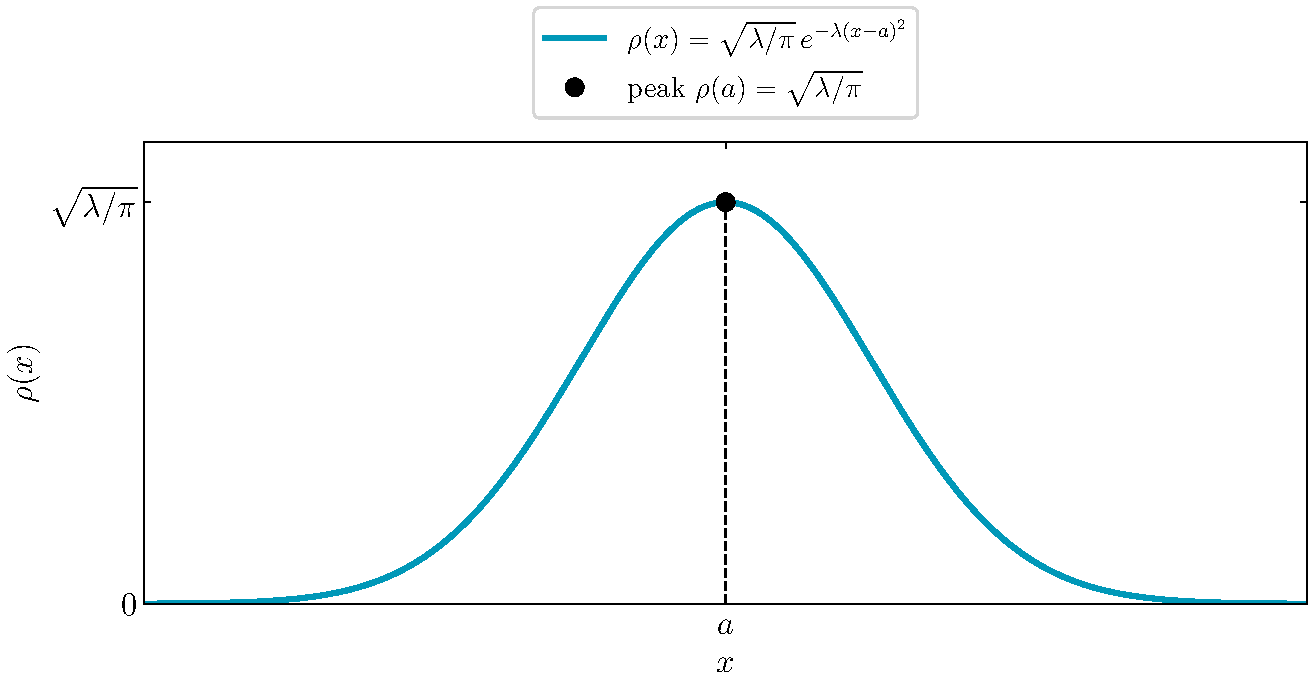
\includegraphics[width=0.9\textwidth]{../chap1/chap1ex1.3c.pdf}
\end{enumerate}

\newpage
\subsection{\textsf{1.4 - Normalization}}
% QUESTION 4
\qs{1.4}{At time \( t = 0 \) a particle is represented by the wave function
\[
	\Psi \!\left( x,0 \right) = \begin{cases}
		\displaystyle{A \frac{x}{a}}, & \text{if } 0 \le x \le a, \\[10pt]
		\displaystyle{A \frac{\!\left( b - x \right)}{\!\left( b - a \right)}}, & \text{if } a \le x \le b, \\[10pt]
		0, & \text{otherwise}
	\end{cases} 
\]
where \( A \), \( a \), and \( b \) are constants.
\begin{enumerate}[label=(\alph*)]
	\item Normalize \( \Psi \) (that is, find \( A \), in terms of \( a \) and \( b \)).
	\item Sketch \( \Psi \!\left( x,0 \right) \), as a function of \( x \).
	\item Where is the particle most likely to be found, at \( t = 0 \)?
	\item What is the probability of finding the particle to the left of \( a \)? Check your result in the limiting cases \( b = a \) and \( b = 2a \).
	\item What is the expectation value of \( x \)?
\end{enumerate}}

\begin{enumerate}[label=(\alph*)]
	\item Normalizing the square-integrable wave function requires
	\begin{align*}
		\int^{b}_{0} \abs{\Psi \!\left( x,0 \right)}^{2} \, dx & = \int^{b}_{0} \Psi^{*}\Psi \, dx \\
								       & = \abs{A}^{2} \!\left[ \int^{a}_{0} \!\left( \frac{x}{a} \right)^{2} \, dx + \int^{b}_{a} \!\left( \frac{b - x}{b - a} \right)^{2} \, dx \right] \\
													 & = 1
	\end{align*}
	We start by computing the integrals, which gets you
	\begin{align*}
		\int^{a}_{0} \!\left( \frac{x}{a} \right)^{2} \, dx + \int^{b}_{a} \!\left( \frac{b - x}{b - a} \right)^{2} \, dx & = \frac{x^{3}}{3a^{2}}\bigg|^{a}_{0} - \frac{\!\left( b - x \right)^{3}}{3 \!\left( b - a \right)^{2}}\bigg|^{b}_{a} \\
		 & = \frac{a}{3} + \frac{b - a}{3} \\ 
		 & = \frac{b}{3}
	\end{align*}
	and leads to
	\[
		\abs{A}^{2} = \frac{3}{b} \quad \implies \quad \abs{A} = A = \sqrt{\frac{3}{b}} 
	\]
	where we select the positive root by convention.
	\item 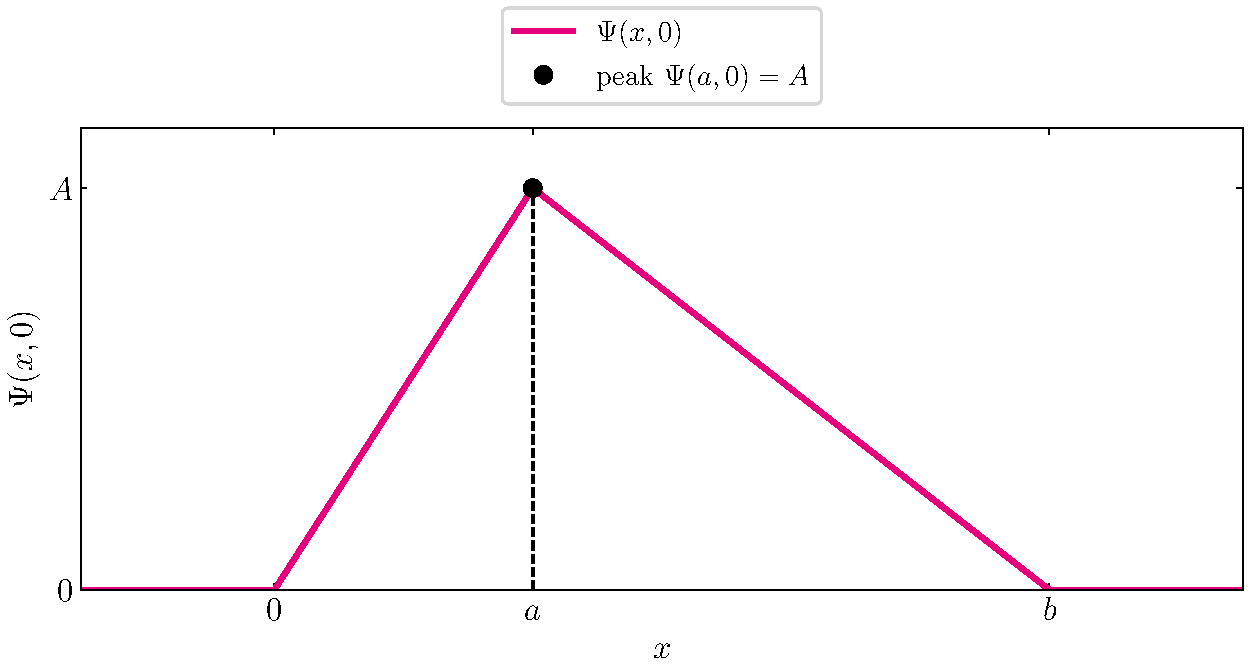
\includegraphics[width=0.9\textwidth]{../chap1/chap1ex1.4b.pdf}
\item From the plot in part (b), the particle is most likely to be found at \( x = a \); since \( \Psi \!\left( x,0 \right) \ge 0 \), it follows that \( \argmax_{x} \Psi(x,0) = \argmax_{x} \abs{\Psi(x,0)}^{2} = a \).
	\item The probability that the particle is found within \( 0 \le x \le a \) is given by integrating \( \abs{\Psi \!\left( x,0 \right)}^{2} \) over that interval:
	\[
		P \!\left( 0 \le x \le a \right) = \frac{3}{b}\int^{a}_{0} \!\left( \frac{x}{a} \right)^{2} \, dx = \frac{3}{b}\!\left( \frac{x^{3}}{3a^{2}} \right)\bigg|^{a}_{0} = \frac{a}{b}
	\]
	When \( a = b \), \( P = 1 \), which is physically sensible as the particle must fall within \( \!\left[ 0,b \right] \). When \( a = b/2 \), \( P = 1/2 \), and \( \Psi \!\left( x,0 \right) \) is an isosceles triangle bisected down \( x = b/2 \).
	\item Derive
	\begin{align*}
		\braket{x} & = \int^{b}_{a} x \!\left( \Psi^{*}\Psi \right) \, dx  \\
			   & = \frac{3}{b}\!\left[ \int^{a}_{0} x \!\left( \frac{x}{a} \right)^{2} \, dx + \int^{b}_{a} x \!\left( \frac{b - x}{b - a} \right)^{2} \, dx \right] \\
			   & = \frac{3}{b} \!\left[ \frac{x^{4}}{4a^{2}}\bigg|^{a}_{0} - \frac{1}{\!\left( b - a \right)^{2}}\!\left( \frac{b \!\left( b - x \right)^{3}}{3} - \frac{\!\left( b - x \right)^{4}}{4} \right)\bigg|^{b}_{a} \right] \\
			   & = \frac{3}{b}\!\left( \frac{a^{2}}{4} + \frac{b \!\left( b - a \right)}{3} - \frac{\!\left( b - a \right)^{2}}{4} \right) \\
			   & = \frac{1}{4b}\!\left( 3a^{2} + 4b^{2} - 4ab - 3b^{2} + 6ab - 3a^{2} \right) \\
			   & = \frac{2ab + b^{2}}{4b} \\
			   & = \frac{2a + b}{4}
	\end{align*}
\end{enumerate}

% QUESTION 5
\qs{1.5}{Consider the wave function
\[
	\Psi \!\left( x,t \right) = Ae^{-\lambda \abs{x}}e^{-i \omega t} 
\]
where \( A \), \( \lambda \), and \( \omega \) are positive real constants. (We'll see in Chapter 2 what potential (\( V \)) actually produces such a wave function.)
\begin{enumerate}[label=(\alph*)]
	\item Normalize \( \Psi \).
	\item Determine the expectation values of \( x \) and \( x^{2} \).
	\item Find the standard deviation of \( x \). Sketch the graph of \( \abs{\Psi}^{2} \), as a function of \( x \), and mark the points \( \left( \braket{x} + \sigma \right) \) and \( \!\left( \braket{x} - \sigma \right) \), to illustrate the sense in which \( \sigma \) represents the ``spread'' in \( x \). What is the probability that the particle would be found outside this range?
\end{enumerate}}

\begin{enumerate}[label=(\alph*)]
	\item We require
	\begin{align*}
		\int^{\infty}_{-\infty} \abs{\Psi \!\left( x,t \right)}^{2} \, dx & = \int^{\infty}_{-\infty} \Psi^{*}\Psi \, dx \\
							 & = \abs{A}^{2}\int^{\infty}_{-\infty} \!\left( e^{-\lambda \abs{x}}e^{-i \omega t} \right) \!\left( e^{-\lambda \abs{x}}e^{i \omega t} \right)\, dx \\
							 & = 2 \abs{A}^{2}\int^{\infty}_{0} e^{-2 \lambda x} \, dx \\
						         & = 1
	\end{align*}
	Solving for \( A \) yields
	\begin{align*}
		2 \abs{A}^{2}\int^{\infty}_{0} e^{-2 \lambda x} \, dx & = -\abs{A}^{2}\frac{e^{-2 \lambda x}}{\lambda}\bigg|^{\infty}_{0} \\
							      & = \frac{\abs{A}^{2}}{\lambda} = 1 \\
		\implies A & = \sqrt{\lambda}
	\end{align*}
	where by premise, \( A \) is positive.
	\item Compute
	\begin{align*}
		\braket{x} & = \lambda\int^{\infty}_{-\infty} x \!\left( e^{-\lambda \abs{x}}e^{-i \omega t} \right)\!\left( e^{-\lambda \abs{x}}e^{i \omega t} \right) \, dx \\
		 & = \lambda\int^{\infty}_{-\infty} xe^{-2 \lambda \abs{x}} \, dx \\ 
		 & = 0 \\
		\braket{x^{2}} & = \lambda\int^{\infty}_{-\infty} x^{2} \!\left( e^{-\lambda \abs{x}}e^{-i \omega t} \right)\!\left( e^{-\lambda \abs{x}}e^{i \omega t} \right) \, dx \\
			       & = 2 \lambda \int^{\infty}_{0} x^{2}e^{-2 \lambda x} \, dx \\
			       & = -e^{-2 \lambda x}\!\left( x^{2} + \frac{x}{\lambda} + \frac{1}{2 \lambda^{2}} \right)\bigg|^{\infty}_{0} \\
			       & = \frac{1}{2 \lambda^{2}}
	\end{align*}
	where antisymmetry about the origin causes the mean \( \braket{x} \) to vanish and integration by parts leads to the result for \( \braket{x^{2}} \).
	\item Derive the standard deviation as 
	\[
		\sigma = \sqrt{\braket{x^{2}} - \braket{x}^{2}} = \frac{1}{\sqrt{2} \lambda} 
	\]
	Plotting the probability density: 
	\begin{center}
	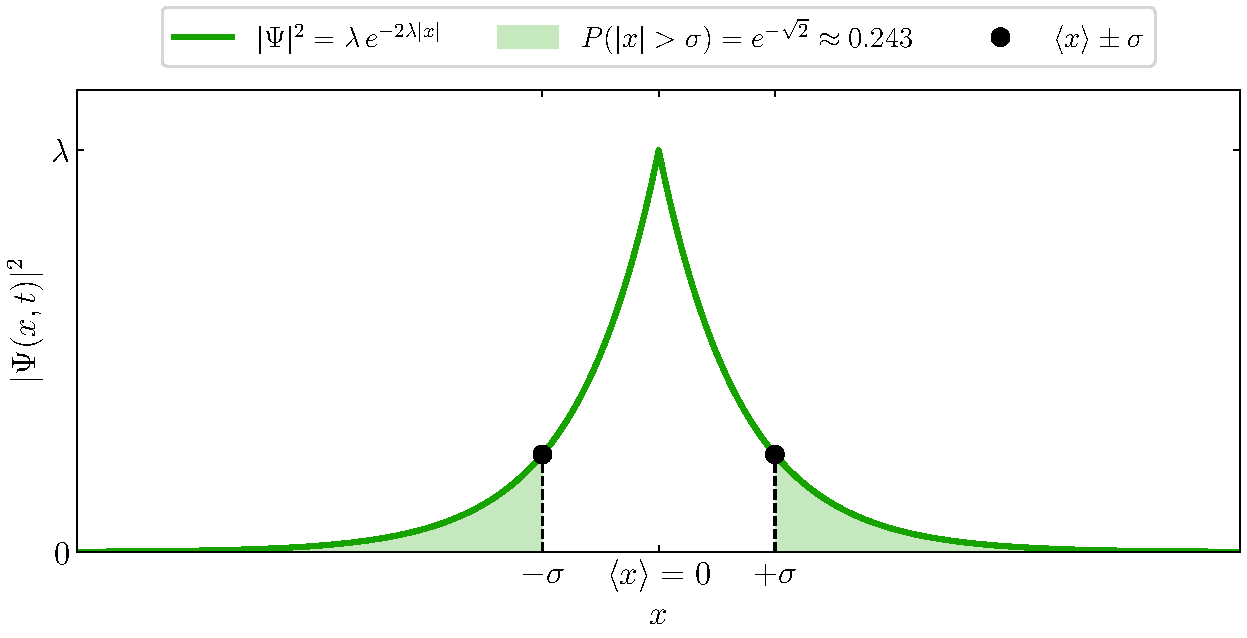
\includegraphics[width=0.9\textwidth]{../chap1/chap1ex1.5c.pdf}
	\end{center}
	It is easy to see that appealing to the symmetry of the density, the probability that the particle is found beyond one standard deviation of the mean is
	\begin{align*}
		P \!\left( \sigma \le x \right) + P \!\left( x \le -\sigma \right) & = 2 \lambda\int^{\infty}_{+\sigma} e^{-2 \lambda x} \, dx \\
		 & = -e^{-2 \lambda x}\Big|^{\infty}_{+\sigma} \\ 
		 & = e^{-\sqrt{2}} \approx 0.243
	\end{align*}
\end{enumerate}

\newpage
\subsection{\textsf{1.5 - Momentum}}
% QUESTION 6
\qs{1.6}{Why can't you do integration-by-parts directly on the middle expression in Equation 1.29 -- pull the time derivative over onto \( x \), note that \( \partial x / \partial t = 0 \), and conclude that \( d \braket{x} / dt = 0 \)?}

Equation 1.29 says
\[
	\frac{d \braket{x}}{d t} = \int x \frac{\partial }{\partial t}\abs{\Psi}^{2} \, dx = \frac{i \hbar}{2m}\int x \frac{\partial }{\partial x}\!\left( \Psi^{*}\frac{\partial \Psi}{\partial x} - \frac{\partial \Psi^{*}}{\partial x}\Psi \right) \, dx 
\]
Consider the product rule
\[
	\frac{\partial }{\partial t}\!\left( x \abs{\Psi}^{2} \right) = \abs{\Psi}^{2}\frac{\partial x}{\partial t} + x \frac{\partial \abs{\Psi}^{2}}{\partial t} = x \frac{\partial }{\partial t}\abs{\Psi}^{2}
\]
In this case, \( x \) is not parameterized by \( t \), so \( \partial x / \partial t = 0 \), but the second term still remains. Our variable of integration, however, is \( x \), \textit{not} \( t \). If we were to integrate over \( x \):
\[
	\frac{d \braket{x}}{d t} = \int \frac{\partial }{\partial t}\!\left( x \abs{\Psi}^{2} \right) \, dx = \int x \frac{\partial }{\partial t}\abs{\Psi}^{2} \, dx
\]
which merely returns us to the middle part of Equation 1.29. On this alone, we would not be able to conclude that the last term is zero, and as such, we cannot conclude \( d \braket{x} / dt = 0 \).

\newpage

% QUESTION 7
\qs{1.7}{Calculate \( d \braket{p} / dt \). \textit{Answer}:
\[
	\frac{d \braket{p}}{d t} = \braket{-\frac{\partial V}{\partial x}} 
\]
Equations 1.32 (or the first part of 1.33) and 1.38 are instances of \textbf{Ehrenfest's theorem}, which tells us that \textit{expectation values obey classical laws}.}

Compute, by way of Leibniz's rule
\begin{align*}
	\frac{d \braket{p}}{d t} & = -i \hbar \frac{d }{d t}\int \Psi^{*}\frac{\partial \Psi}{\partial x} \, dx = -i \hbar \int \frac{\partial }{\partial t}\!\left( \Psi^{*}\frac{\partial \Psi}{\partial x} \right) \, dx \\
				 & = -i \hbar \int \!\left( \frac{\partial \Psi^{*}}{\partial t}\frac{\partial \Psi}{\partial x} + \Psi^{*}\underbrace{\frac{\partial }{\partial t}\frac{\partial \Psi}{\partial x}}_{= \frac{\partial }{\partial x}\frac{\partial \Psi}{\partial t}} \right) \, dx \\ 
				 & = -i \hbar \int \!\left[ \!\left( -\frac{i \hbar}{2m}\frac{\partial^2 \Psi^{*}}{\partial x^2} + \frac{i}{\hbar}V \Psi^{*} \right)\frac{\partial \Psi}{\partial x} + \Psi^{*}\frac{\partial }{\partial x}\!\left( \frac{i \hbar}{2m}\frac{\partial^2 \Psi}{\partial x^2} - \frac{i}{\hbar}V \Psi \right) \right] \, dx \\
	 & = -\frac{\hbar^{2}}{2m}\int \!\left( \frac{\partial^2 \Psi^{*}}{\partial x^2}\frac{\partial \Psi}{\partial x} - \Psi^{*}\frac{\partial^3 \Psi}{\partial x^3} \right) \, dx + \int \!\left( V \Psi^{*}\frac{\partial \Psi}{\partial x} - \Psi^{*}\frac{\partial }{\partial x}\!\left( V \Psi \right) \right) \, dx \\
	 & = \int \!\left[ \underbrace{\!\left( V \Psi^{*}\frac{\partial \Psi}{\partial x} - V \Psi^{*}\frac{\partial \Psi}{\partial x} \right)}_{= 0} - \Psi^{*}\Psi \frac{\partial V}{\partial x} \right] \, dx \\
	 & = -\int \frac{\partial V}{\partial x}\abs{\Psi}^{2} \, dx \\
	 & = \braket{-\frac{\partial V}{\partial x}}
\end{align*}
where in going from the fourth line to the fifth we use the fact that \( \Psi, \Psi^{*} \rightarrow 0 \) along with their first derivative as \( x \rightarrow \pm \infty \).

\vspace{12pt}

% QUESTION 8
\qs{1.8}{Suppose you add a constant \( V_{0} \) to the potential energy (by ``constant'' I mean independent of \( x \) as well as \( t \)). In \textit{classical} mechanics this doesn't change anything, but what about \textit{quantum mechanics}? Show that the wave function picks up a time-dependent phase factor: \( \exp \!\left( -iV_{0}t / \hbar \right) \). What effect does this have on the expectation value of a dynamical variable?}

In essence, we wish to prove that for the Schr\"odinger equation with an added constant potential energy term
\[
	i \hbar \frac{\partial \tilde{\Psi}}{\partial t} = -\frac{\hbar^{2}}{2m}\frac{\partial^2 \tilde{\Psi}}{\partial x^2} + \!\left( V + V_{0} \right)\tilde{\Psi} 
\]
we have a solution with a time-dependent phase factor
\[
	\tilde{\Psi} = \Psi e^{-iV_{0}t / \hbar} 
\]
First compute
\begin{align*}
	\frac{\partial \tilde{\Psi}}{\partial t} & = \frac{\partial \Psi}{\partial t}e^{-iV_{0}t / \hbar} - \frac{iV_{0}}{\hbar}\Psi e^{-iV_{0}t / \hbar} \\
	\frac{\partial^2 \tilde{\Psi}}{\partial x^2} & = \frac{\partial^2 \Psi}{\partial x^2}e^{-iV_{0}t / \hbar}
\end{align*}
Then substitute into Schr\"odinger's equation and cancel the \( e^{-iV_{0}t / \hbar} \) terms:
\[
	i \hbar \frac{\partial \Psi}{\partial t} + V_{0}\Psi = -\frac{\hbar^{2}}{2m}\frac{\partial^2 \Psi}{\partial x^2} + \!\left( V + V_{0} \right)\Psi 
\]
and canceling the \( V_{0}\Psi \) terms restores the original Schr\"odinger's equation, as desired. Referring to equation 1.36 for the expectation value of any dynamical quantity:
\[
	\braket{Q \!\left( x,p \right)} = \int \Psi^{*}Q \!\left( x,\frac{\hbar}{i}\frac{\partial }{\partial x} \right)\Psi \, dx 
\]
And substituting \( \tilde{\Psi} \), bearing in mind that the time-dependent phase factor is exclusively in \( t \) and thus treated as a constant in the integral over \( x \), we find
\begin{align*}
	\braket{Q \!\left( x,p \right)} & = \int \tilde{\Psi}^{*}Q \!\left( x,\frac{\hbar}{i}\frac{\partial }{\partial x} \right)\tilde{\Psi} \, dx \\
					& = \int \underbrace{\Psi^{*}e^{iV_{0}t / \hbar}}Q \!\left( x,\frac{\hbar}{i}\frac{\partial }{\partial x} \right)\underbrace{\Psi e^{-iV_{0}t / \hbar}} \, dx \\
					& = \int \Psi^{*}Q \!\left( x,\frac{\hbar}{i}\frac{\partial }{\partial x} \right)\Psi \, dx
\end{align*}
meaning that expectation values are \textbf{unchanged} by the presence of a constant potential energy.

\newpage
\subsection{\textsf{1.6 - The Uncertainty Principle}}
% QUESTION 9
\qs{1.9}{A particle of mass \( m \) is in the state
\[
	\Psi \!\left( x,t \right) = Ae^{-a \!\left[ \!\left( mx^{2} / \hbar \right) + it \right]} 
\]
where \( A \) and \( a \) are positive real constants.
\begin{enumerate}[label=(\alph*)]
	\item Find \( A \).
	\item For what potential energy function \( V \!\left( x \right) \) does \( \Psi \) satisfy the Schr\"odinger equation?
	\item Calculate the expectation values of \( x \), \( x^{2} \), \( p \), and \( p^{2} \).
	\item Find \( \sigma_{x} \) and \( \sigma_{p} \). Is their product consistent with the uncertainty principle?
\end{enumerate}}
\begin{enumerate}[label=(\alph*)]
	\item Normalize to derive
	\begin{align*}
		\int^{\infty}_{-\infty} \Psi^{*}\Psi \, dx & = \abs{A}^{2}\int^{\infty}_{-\infty} \!\left( e^{-a \!\left[ \!\left( mx^{2} / \hbar \right) - it \right]} \right)\!\left( e^{-a \!\left[ \!\left( mx^{2} / \hbar \right) + it \right]} \right) \, dx \\
							   & =  \abs{A}^{2}\int^{\infty}_{-\infty} e^{-2amx^{2} / \hbar} \, dx \\
							   & = \abs{A}^{2}\sqrt{\frac{\pi \hbar}{2am}} = 1 \\
							\implies A & = \!\left( \frac{2am}{\pi \hbar} \right)^{1/4}
	\end{align*}
	\item Compute
	\begin{align*}
		\frac{\partial \Psi}{\partial t} & = -ai \Psi \\
		\frac{\partial \Psi}{\partial x} & = -\frac{2am}{\hbar}x \Psi \\ 
		\frac{\partial^2 \Psi}{\partial x^2} & = \!\left( -\frac{2am}{\hbar} + \frac{4a^{2}m^{2}}{\hbar^{2}}x^{2} \right)\Psi
	\end{align*}
	Substituting into Schr\"odinger's equation produces
	\[
		a \hbar \Psi = \!\left( a \hbar - 2a^{2}m x^{2} \right)\Psi + V \!\left( x \right) \Psi 
	\]
	Canceling \( \Psi \) throughout and rearranging to solve \( V \!\left( x \right) \), we have
	\[
		V \!\left( x \right) = 2a^{2}mx^{2} 
	\]
	\item Using the result of problem 1.8, we need not consider the phase factor. From equation 1.36 the expectations are
	\begin{align*}
		\braket{x} & = \int^{\infty}_{-\infty} \Psi^{*}x \Psi \, dx = \abs{A}^{2}\int^{\infty}_{-\infty} xe^{-\alpha x^{2}} \, dx \\
			   & = 0 \\
		\braket{x^{2}} & = \int^{\infty}_{-\infty} \Psi^{*}x^{2}\Psi \, dx = \abs{A}^{2}\int^{\infty}_{-\infty} x^{2}e^{-\alpha x^{2}} \, dx = 2 \abs{A}^{2}\int^{\infty}_{0} x^{2}e^{-\alpha x^{2}} \, dx \\
			       & = \frac{\abs{A}^{2}}{2 \alpha}\sqrt{\frac{\pi}{\alpha}} \\
		\braket{p} & = \int^{\infty}_{-\infty} \Psi^{*}\frac{\hbar}{i}\frac{\partial \Psi}{\partial x} \, dx = -\frac{2 \abs{A}^{2}am}{i}\int^{\infty}_{-\infty} xe^{-\alpha x^{2}} \, dx \\
			   & = 0 \\
		\braket{p^{2}} & = -\hbar^{2}\int^{\infty}_{-\infty} \Psi^{*}\frac{\partial^2 \Psi}{\partial x^2} \, dx \\
			       & = -\abs{A}^{2}\hbar^{2}\int^{\infty}_{-\infty} \!\left( -\alpha + \alpha^{2}x^{2} \right)e^{-\alpha x^{2}} \, dx \\
			       & = \abs{A}^{2} \!\left[ \alpha \hbar^{2}\int^{\infty}_{-\infty} e^{-\alpha x^{2}} \, dx - 2 \alpha^{2}\hbar^{2}\int^{\infty}_{0} x^{2}e^{-\alpha x^{2}} \, dx \right]  \\
			       & = \abs{A}^{2} \!\left[ \alpha \hbar^{2}\sqrt{\frac{\pi}{\alpha}} - \frac{\alpha \hbar^{2}}{2}\sqrt{\frac{\pi}{\alpha}} \right] \\
			       & = \frac{\abs{A}^{2}\alpha \hbar^{2}}{2}\sqrt{\frac{\pi}{\alpha}}
	\end{align*}
	where \( \alpha = 2am / \hbar \). Simplifying the nonzero expecations gives us 
	\begin{align*}
		\braket{x^{2}} & = \frac{1}{2}\!\left( \frac{2am}{\pi \hbar} \right)^{1/2}\!\left( \frac{\hbar}{2am} \right)^{3/2}\sqrt{\pi} = \frac{\hbar}{4am} \\
		\braket{p^{2}} & = \frac{1}{2}\!\left( \frac{2am}{\pi \hbar} \right)^{1/2}\!\left( \frac{2am}{\hbar} \right)^{1/2}\hbar^{2}\sqrt{\pi} = am \hbar
	\end{align*}
	\item Since \( \braket{x} = \braket{p} = 0 \), 
	\begin{align*}
		\sigma_{x} & = \sqrt{\frac{\hbar}{4am}} \\
		\sigma_{p} & = \sqrt{am \hbar}
	\end{align*}
	We can conclude
	\[
		\sigma_{x}\sigma_{p} = \frac{\hbar}{2}
	\]
	which is beautifully consistent with the uncertainty principle. This is the wave function corresponding to the quantum harmonic oscillator in its ground-state (more on this in chapter 2).
\end{enumerate}

\newpage
\subsection{\textsf{Further Problems for Chapter 1}}
% QUESTION 10
\qs{1.10}{Consider the first 25 digits in the decimal expansion of \( \pi \) (3, 1, 4, 1, 5, 9, ...).
\begin{enumerate}[label=(\alph*)]
	\item If you selected one number at random, from this set, what are the probabilities of getting each of the 10 digits?
	\item What is the most probable digit? What is the median digit? What is the average value?
	\item Find the standard deviation for this distribution.
\end{enumerate}}

\begin{enumerate}[label=(\alph*)]
	\item \begin{table}[h]
	\centering
	\begin{tabular}{c c}
		\hline
		Digit \( j \) & \( P \!\left( j \right) \) \\
		\hline
		0 & \( 0 \) \\
		1 & \( 2/25 \) \\
		2 & \( 3/25 \) \\
		3 & \( 5/25 \) \\
		4 & \( 3/25 \) \\
		5 & \( 3/25 \) \\
		6 & \( 3/25 \) \\
		7 & \( 1/25 \) \\
		8 & \( 2/25 \) \\
		9 & \( 3/25 \) \\
		\hline
	\end{tabular}
	\end{table}
	\item The most probable digit is \( 3 \), with \( P \!\left( 3 \right) = 1/5 \), with median digit \( 4 \), and average value
	\begin{align*}
		\braket{j} & = \sum j P \!\left( j \right) \\
			   & = \frac{1 \cdot 2 + 2 \cdot 3 + 3 \cdot 5 + 4 \cdot 3 + 5 \cdot 3 + 6 \cdot 3 + 7 \cdot 1 + 8 \cdot 2 + 9 \cdot 3}{25} \\
			   & = \frac{118}{25} = 4.72
	\end{align*}
	\item Compute the mean of \( j^{2} \):
	\begin{align*}
		\braket{j^{2}} & = \sum j^{2}P \!\left( j \right) \\
			   & = \frac{1^{2} \cdot 2 + 2^{2} \cdot 3 + 3^{2} \cdot 5 + 4^{2} \cdot 3 + 5^{2} \cdot 3 + 6^{2} \cdot 3 + 7^{2} \cdot 1 + 8^{2} \cdot 2 + 9^{2} \cdot 3}{25} \\
			   & = \frac{710}{25} = 28.4
	\end{align*}
	Then the standard deviation is
	\[
		\sigma = \sqrt{\braket{j^{2}} - \braket{j}^{2}} = \sqrt{28.4 - 4.72^{2}} = \sqrt{6.1216} \approx 2.474
	\]
\end{enumerate}

% QUESTION 11
\qs{1.11}{The needle on a broken car speedometer is free to swing, and bounces perfectly off the pins on either end, so that if you give it a flick it is equally likely to come to rest at any angle between \( 0 \) and \( \pi \).
\begin{enumerate}[label=(\alph*)]
	\item What is the probability density, \( \rho \!\left( \theta \right) \)? \textit{Hint}: \( \rho \!\left( \theta \right) \, d \theta \) is the probability that the needle will come to rest between \( \theta \) and \( \!\left( \theta + d \theta \right) \). Graph \( \rho \!\left( \theta \right) \) as a function of \( \theta \), from \( -\pi / 2 \) to \( 3 \pi / 2 \). (Of course, \textit{part} of this interval is excluded, so \( \rho \) is zero there.) Make sure that the total probability is 1.
	\item Compute \( \braket{\theta} \), \( \braket{\theta^{2}} \), and \( \sigma \), for this distribution.
	\item Compute \( \braket{\sin\!\left(\theta\right)} \), \( \braket{\cos\!\left(\theta\right)} \), and \( \braket{\cos^{2}\!\left(\theta\right)} \).
\end{enumerate}}

\begin{enumerate}[label=(\alph*)]
	\item The density is given by
	\[
		\rho \!\left( \theta \right) = \begin{cases}
			\displaystyle{\frac{1}{\pi}}, & 0 \le \theta \le \pi \\[10pt]
			0, & -\pi / 2 \le \theta < 0 \text{ or } \pi < \theta \le 3 \pi / 2
		\end{cases}
	\]
	Confirm that the total probability is 1:
	\[
		\int^{\pi}_{0} \frac{d \theta}{\pi} = \frac{\theta}{\pi}\bigg|^{\pi}_{0} = 1  
	\]
	Graph the density as 
	\begin{center}
	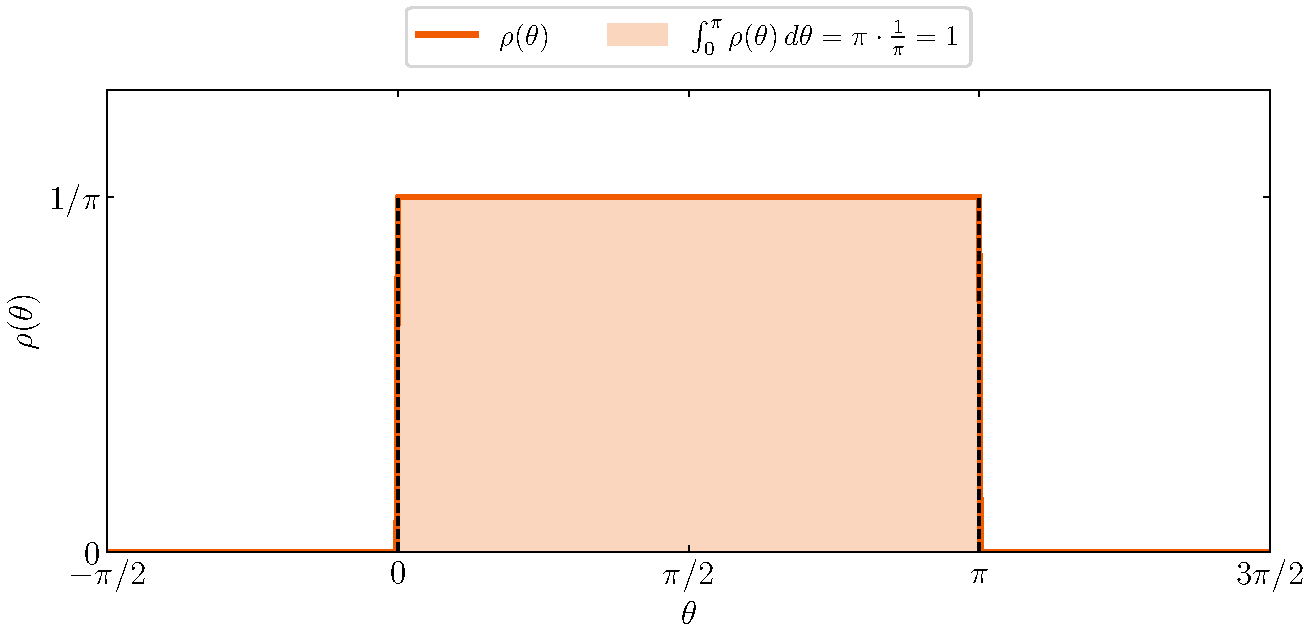
\includegraphics[width=0.9\textwidth]{../chap1/chap1ex1.11a.pdf}
	\end{center}
	But we ought not to be satisfied by theory alone. We can empirically simulate this experiment and find the ensuing histogram conforms to our theoretical result:
	\begin{center}
	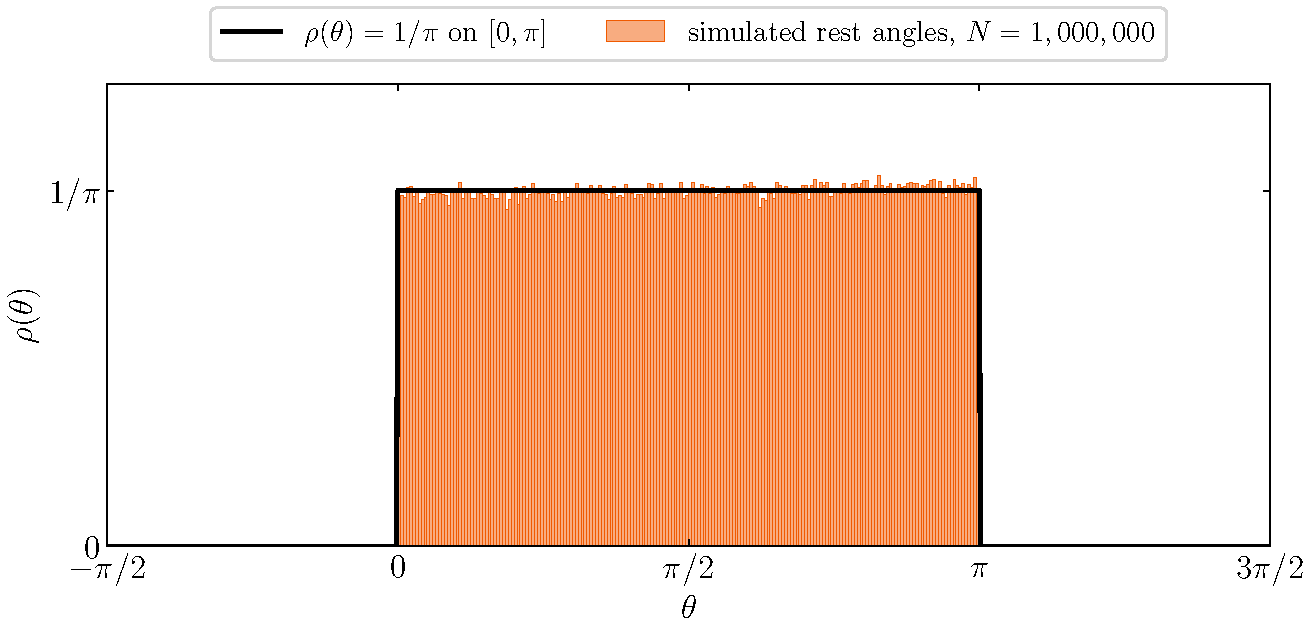
\includegraphics[width=0.9\textwidth]{../chap1/chap1ex1.11a_sim.pdf}
	\end{center}
	\item Compute
	\begin{align*}
		\braket{\theta} & = \int^{\pi}_{0} \frac{\theta}{\pi} \, d \theta = \frac{\theta^{2}}{2 \pi}\bigg|^{\pi}_{0} = \frac{\pi}{2} \\
		\braket{\theta^{2}} & = \int^{\pi}_{0} \frac{\theta^{2}}{\pi} \, d \theta = \frac{\theta^{3}}{3 \pi}\bigg|^{\pi}_{0} = \frac{\pi^{2}}{3} \\ 
		\sigma & = \sqrt{\braket{\theta^{2}} - \braket{\theta}^{2}} = \sqrt{\frac{\pi^{2}}{3} - \frac{\pi^{2}}{4}} = \frac{\pi}{2 \sqrt{3}}
	\end{align*}
	\item Compute
	\begin{align*}
		\braket{\sin\!\left(\theta\right)} & = \int^{\pi}_{0} \frac{\sin\!\left(\theta\right)}{\pi} \, d \theta = -\frac{\cos\!\left(\theta\right)}{\pi}\bigg|^{\pi}_{0} = \frac{2}{\pi} \\
		\braket{\cos\!\left(\theta\right)} & = \int^{\pi}_{0} \frac{\cos\!\left(\theta\right)}{\pi} \, d \theta = \frac{\sin\!\left(\theta\right)}{\pi}\bigg|^{\pi}_{0} = 0 \\ 
		\braket{\cos^{2}\!\left(\theta\right)} & = \int^{\pi}_{0} \frac{\cos^{2}\!\left(\theta\right)}{\pi} \, d \theta = \int^{\pi}_{0} \!\left( \frac{1 + \cos\!\left(2 \theta\right)}{2 \pi} \right) \, d \theta \\
						       & = \frac{\theta}{2 \pi}\bigg|^{\pi}_{0} + \frac{\sin\!\left(2 \theta\right)}{4 \pi}\bigg|^{\pi}_{0} = \frac{1}{2}
	\end{align*}
\end{enumerate}

\newpage
% QUESTION 12
\qs{1.12}{We consider the same device as the previous problem, but this time we are interested in the \( x \)-coordinate of the needle point -- that is, the ``shadow,'' or ``projection,'' of the needle on the horizontal line.
\begin{enumerate}[label=(\alph*)]
	\item What is the probability density \( \rho \!\left( x \right) \)? Graph \( \rho \!\left( x \right) \) as a function of \( x \), from \( -2r \) to \( +2r \), where \( r \) is the length of the needle. Make sure the total probability is 1. \textit{Hint}: \( \rho \!\left( x \right) \, dx \) is the probability that the projection lies between \( x \) and \( x + dx \). You know (from Problem 1.11) the probability that \( \theta \) is in a given range; the question is, what interval \( dx \) corresponds to the interval \( d \theta \)?
	\item Compute \( \braket{x} \), \( \braket{x^{2}} \), and \( \sigma \), for this distribution. Explain how you could have obtained these results from part (c) of Problem 1.11.
\end{enumerate}}

\begin{enumerate}[label=(\alph*)]
	\item Begin with the polar coordinate definition \( x = r \cos\!\left(\theta\right) \). In fact, this is our projection of the needle onto the horizontal axis. Take the inverse: \( \theta = \cos^{-1}\!\left(x / r\right) \). The relation between \( dx \) and \( d \theta \) is
	\[
		d \theta = -\frac{1}{r}\frac{1}{\sqrt{1 - x^{2} / r^{2}}}dx = -\frac{dx}{\sqrt{r^{2} - x^{2}}}, \quad \abs{x} < r
	\]
	Taking the probability density of problem 1.11, we substitute our differential and bounds (\( \theta = \pi \rightarrow x = -r \) and \( \theta = 0 \rightarrow x = r \)) to derive
	\[
		 -\int^{-r}_{r} \frac{dx}{\pi \sqrt{r^{2} - x^{2}}} = \int^{r}_{-r} \frac{dx}{\pi \sqrt{r^{2} - x^{2}}} = 1
	\]
	and since we merely make a bijection \( \theta \mapsto x = r \cos\!\left(\theta\right) \) between the range \( \!\left[ 0,\pi \right] \rightarrow \!\left[ -r,r \right] \), we conclude our probability density (in Cartesian coordinates) is
	\[
		\rho \!\left( x \right) = \begin{cases}
			1 / \pi \sqrt{r^{2} - x^{2}}, & -r < x < r \\
			0, & \text{otherwise} 
		\end{cases} 
	\]
	We graph the density and simulate this experiment below:
	\begin{center}
	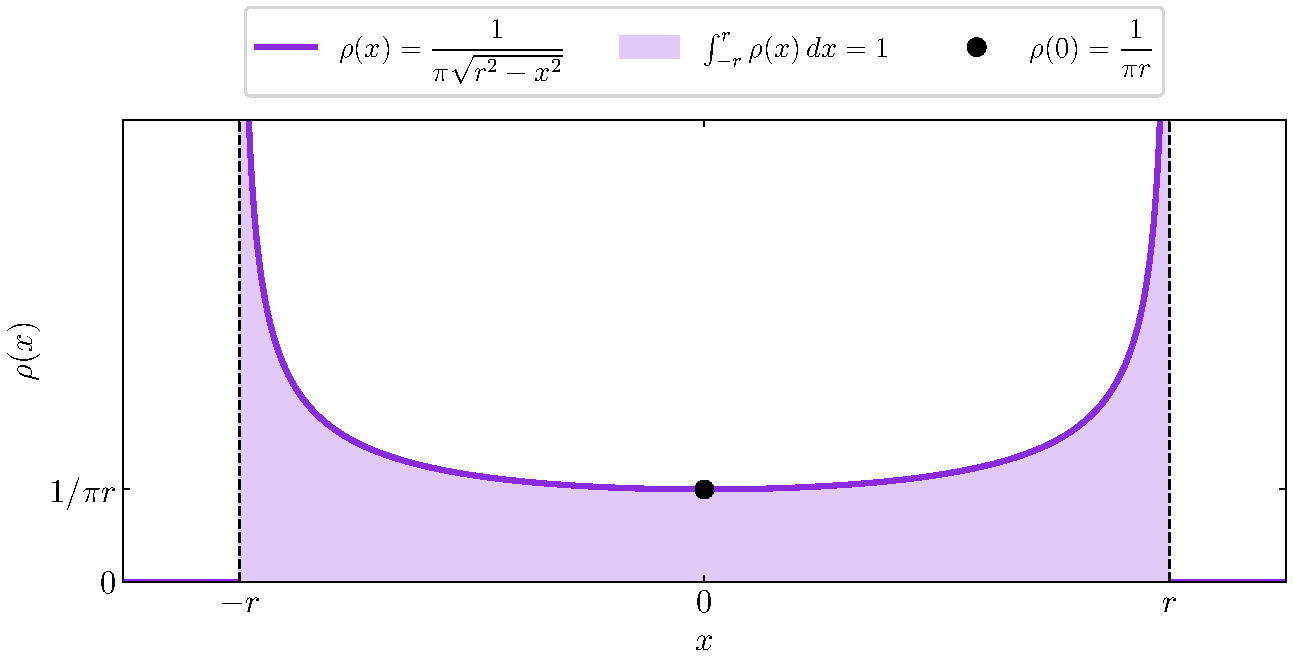
\includegraphics[width=0.8\textwidth]{../chap1/chap1ex1.12.pdf}
	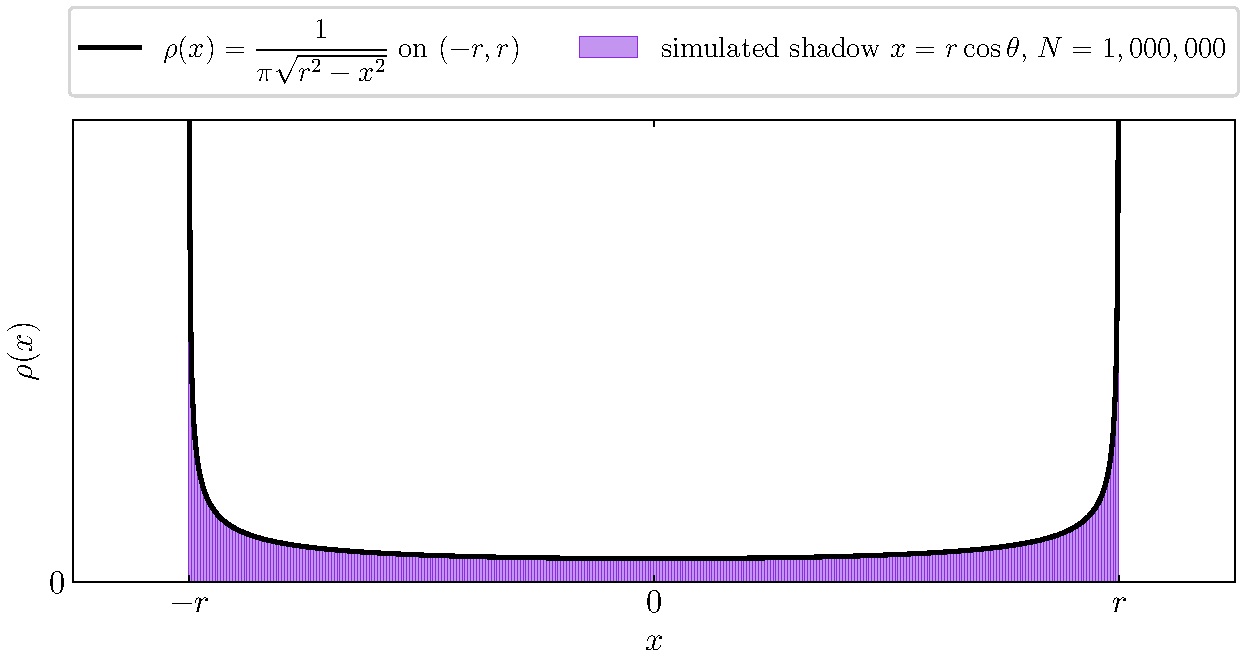
\includegraphics[width=0.8\textwidth]{../chap1/chap1ex1.12_sim.pdf}
	\end{center}
	\item Compute
	\begin{align*}
		\braket{x} & = \int^{r}_{-r} \frac{x}{\pi \sqrt{r^{2} - x^{2}}} \, dx = 0 \quad (\text{by oddness of the integrand}) \\
		\braket{x^{2}} & = \int^{r}_{-r} \frac{x^{2}}{\pi \sqrt{r^{2} - x^{2}}} \, dx = \frac{1}{\pi}\!\left[ \frac{r^{2}}{2}\arcsin\!\left( \frac{x}{r} \right) - \frac{x}{2}\sqrt{r^{2} - x^{2}} \right]\bigg|^{r}_{-r} = \frac{r^{2}}{2} \\ 
		\sigma & = \sqrt{\braket{x^{2}} - \braket{x}^{2}} = \frac{r}{\sqrt{2}}
	\end{align*}
	The simpler approach is to use our relation \( \cos\!\left(\theta\right) = x/r \) and substitute into the expectations computed for \( \cos\!\left(\theta\right) \) and \( \cos^{2}\!\left(\theta\right) \) in the previous problem:
	\begin{align*}
		\braket{\cos\!\left(\theta\right)} & = \braket{\frac{x}{r}} = 0\\
		\braket{\cos^{2}\!\left(\theta\right)} & = \braket{\frac{x^{2}}{r^{2}}} = \frac{1}{2}
	\end{align*}
	where multiplying through by \( r \) and \( r^{2} \) respectively yields the desired answers.
\end{enumerate}

% QUESTION 13
\qs{1.13}{\textbf{Buffon's needle}. A needle of length \( l \) is dropped at random onto a sheet of paper ruled with parallel lines a distance \( l \) apart. What is the probability that the needle will cross a line? \textit{Hint}: Refer to Problem 1.12.}

Some intuition to motivate us:
\begin{itemize}[label=\(\circ\)]
	\item Fundamentally, there are two \textbf{independent} variables: \( \theta \in \!\left[ 0,\pi \right] \), the angle of the needle relative to the lines, and \( y \), the vertical distance between the center of the needle to the nearest line. Assume both are distributed uniformly.
	\item The likelihood that the needle will fall parallel \textbf{and} land on one of the paper's lines is negligible.
	\item The more vertical the needle is, the higher the likelihood it will intersect with one of the lines. More precisely, \( P \!\left( \text{cross} \right) \uparrow \) when \( l \abs{\cos\!\left(\theta\right)} \downarrow \).
\end{itemize}
The vertical height of the needle, which is a function of \( \theta \), is \( l \sin\!\left(\theta\right) \). Then the vertical distance from the center of the needle to either of its ends is \( l \sin\!\left(\theta\right) / 2 \). \textbf{Notably, if the center of the needle falls some vertical distance \( y < l \sin\!\left(\theta\right) / 2 \)}, within the paper's lines, we have an intersection. 

The density \( \rho \!\left( y \right) \) is
\[
	\rho \!\left( y \right) = \frac{1}{l}, \quad 0 \le y \le l
\]
which is easily verified as normalizing to 1. 
Since we have independently distributed variables, the joint probability is given from integrating the product of the corresponding densities for \( \theta \) and \( y \). Given that the events that the center of the needle falls within either \( \!\left[ 0,l \sin\!\left(\theta\right) / 2 \right] \) or \( \!\left[ l - l \sin\!\left(\theta\right) / 2,l \right] \) are disjoint\footnote{With overlap only when \( \theta = \pi / 2 \), which has probability \( P \!\left( \theta = \pi / 2 \right) = 0 \).}, we can simply multiply the densities with bounds \( 0 \le \theta \le \pi \) and \( 0 \le y \le l \sin\!\left(\theta\right) / 2 \) and \( l - l \sin\!\left(\theta\right) / 2 \le y \le l \):
\begin{align*}
	P \!\left( \text{cross} \right) & = \iint \rho \!\left( \theta \right)\rho \!\left( y \right) \, dy \, d \theta \\
					& = \frac{1}{\pi l}\int^{\pi}_{0} \!\left[ \int^{l \sin\!\left(\theta\right) / 2}_{0} dy + \int^{l}_{l - l \sin\!\left(\theta\right) / 2} \, dy \right] \, d \theta \\
										    & = \frac{1}{\pi l}\int^{\pi}_{0} l \sin\!\left(\theta\right) \, d \theta \\
										    & = \frac{2}{\pi}
\end{align*}

For fun, I ran a Monte Carlo simulation of Buffon's needle experiment, demonstrating that by the law of large numbers, as \( N \) tends towards infinity, \( P \!\left( \text{cross} \right) \) approaches \( 2 / \pi \):

\begin{center}
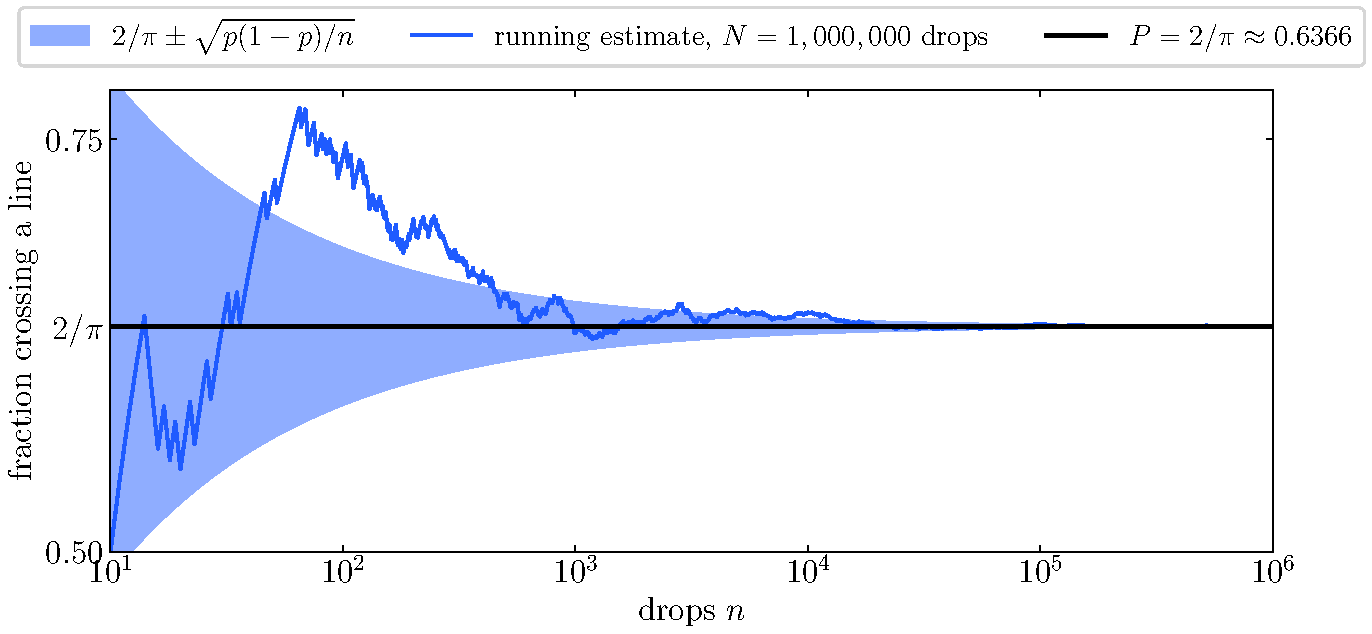
\includegraphics[width=1.0\textwidth]{../chap1/chap1ex1.13_sim.pdf}
\end{center}

\newpage
% QUESTION 14
\qs{1.14}{Let \( P_{ab}\!\left( t \right) \) be the probability of finding a particle in the range \( \!\left( a < x < b \right) \), at time \( t \).
\begin{enumerate}[label=(\alph*)]
	\item Show that
	\[
		\frac{d P_{ab}}{d t} = J \!\left( a,t \right) - J \!\left( b,t \right) 
	\]
	where
	\[
		J \!\left( x,t \right) \equiv \frac{i \hbar}{2m}\!\left( \Psi \frac{\partial \Psi^{*}}{\partial x} - \Psi^{*}\frac{\partial \Psi}{\partial x} \right) 
	\]
	What are the units of \( J \!\left( x,t \right) \)? \textit{Comment}: \( J \) is called the \textbf{probability current}, because it tells you the rate at which probability is ``flowing'' past the point \( x \). If \( P_{ab}\!\left( t \right) \) is increasing, then more probability is flowing into the region at one end than flows out at the other.
	\item Find the probability current for the wave function in Problem 1.9. (This is not a very pithy example, I'm afraid; we'll encounter more substantial ones in due course.)
\end{enumerate}}
\begin{enumerate}[label=(\alph*)]
	\item The probability \( P_{ab}\!\left( t \right) \) is 
	\[
		P_{ab}\!\left( t \right) = \int^{b}_{a} \abs{\Psi \!\left( x,t \right)}^{2} \, dx  
	\]
	By the Leibniz rule,
	\begin{align*}
		\frac{d P_{ab}}{d t} & = \int^{b}_{a} \frac{\partial }{\partial t}\abs{\Psi \!\left( x,t \right)}^{2} \, dx = \int^{b}_{a} \frac{\partial }{\partial t}\!\left( \Psi^{*}\Psi \right) \, dx \\
				     & = \int^{b}_{a} \!\left( \Psi \frac{\partial \Psi^{*}}{\partial t} + \Psi^{*}\frac{\partial \Psi}{\partial t} \right) \, dx \\
				     & = \int^{b}_{a} \!\left[ \Psi \!\left( -\frac{i \hbar}{2m}\frac{\partial^2 \Psi^{*}}{\partial x^2} + \frac{iV}{\hbar}\Psi^{*} \right) + \Psi^{*}\!\left( \frac{i \hbar}{2m}\frac{\partial^2 \Psi}{\partial x^2} - \frac{iV}{\hbar}\Psi \right)  \right] \, dx \\
				     & = \frac{i \hbar}{2m}\int^{b}_{a} \!\left( -\Psi \frac{\partial^2 \Psi^{*}}{\partial x^2} + \Psi^{*}\frac{\partial^2 \Psi}{\partial x^2} \right) \, dx \\
				     & = \frac{i \hbar}{2m}\!\left( -\Psi \frac{\partial \Psi^{*}}{\partial x} + \Psi^{*}\frac{\partial \Psi}{\partial x} \right)\bigg|^{b}_{a} \\
				     & = J \!\left( a,t \right) - J \!\left( b,t \right)
	\end{align*}
	Since \( P_{ab}\!\left( t \right) \), as with any probability, is a unitless quantity, the probability current \( J \!\left( x,t \right) \) has units \( \text{s}^{-1} \). 
	\item From the wave function
	\[
		\Psi \!\left( x,t \right) = Ae^{-a \!\left[ \!\left( mx^{2} / \hbar \right) + it \right]}, \quad A = \!\left( \frac{2am}{\pi \hbar} \right)^{1/4}
	\]
	Compute
	\[
		\frac{\partial \Psi}{\partial x} = -\frac{2Aam}{\hbar}xe^{-a \!\left[ \!\left( mx^{2}/\hbar \right) + it \right]}
	\]
	Then
	\[
		J \!\left( x,t \right) = \frac{i \hbar}{2m}\!\left( -\frac{2A^{2}am}{\hbar}xe^{-2amx^{2}/\hbar} + \frac{2A^{2}am}{\hbar}xe^{-2amx^{2}/\hbar} \right) = 0
	\]
	which physically indicates to us that the wave function is ``stationary'' and \( \abs{\Psi \!\left( x,t \right)}^{2} \) is unchanged for any value of \( x \).
\end{enumerate}

% QUESTION 15
\qs{1.15}{Suppose you wanted to describe an \textbf{unstable particle}, that spontaneously disintegrates with a ``lifetime'' \( \tau \). In that case the total probability of finding the particle somewhere should \textit{not} be constant, but should decrease at (say) an exponential rate:
\[
	P \!\left( t \right) \equiv \int^{\infty}_{-\infty} \abs{\Psi \!\left( x,t \right)}^{2} \, dx = e^{-t/\tau}  
\]
A crude way of achieving this result is as follows. In Equation 1.24 we tacitly assumed that \( V \) (the potential energy) is \textit{real}. That is certainly reasonable, but leads to the ``conservation of probability'' enshrined in Equation 1.27. What if we assign to \( V \) an imaginary part:
\[
	V = V_{0} - i \Gamma 
\]
where \( V_{0} \) is the true potential energy and \( \Gamma \) is a positive real constant?
\begin{enumerate}[label=(\alph*)]
	\item Show that (in place of Equation 1.27) we now get
	\[
		\frac{d P}{d t} = -\frac{2 \Gamma}{\hbar}P 
	\]
	\item Solve for \( P \!\left( t \right) \), and find the lifetime of the particle in terms of \( \Gamma \).
\end{enumerate}}
\begin{enumerate}[label=(\alph*)]
	\item From the adjusted Schr\"odinger equation, we have
	\[
		\frac{\partial \Psi}{\partial t} = \frac{i \hbar}{2m}\frac{\partial^2 \Psi}{\partial x^2} - \frac{i}{\hbar}\!\left( V_{0} - i \Gamma \right)\Psi = \frac{i \hbar}{2m}\frac{\partial^2 \Psi}{\partial x^2} - \!\left( \frac{\Gamma + iV_{0}}{\hbar} \right)\Psi
	\]
	Then the complex conjugate is
	\[
		\frac{\partial \Psi^{*}}{\partial t} = -\frac{i \hbar}{2m}\frac{\partial^2 \Psi^{*}}{\partial x^2} - \!\left( \frac{\Gamma - iV_{0}}{\hbar} \right)\Psi^{*}
	\]
	Using these pieces, we can derive
	\begin{align*}
		\frac{\partial }{\partial t}\abs{\Psi}^{2} & = \Psi^{*}\frac{\partial \Psi}{\partial t} + \frac{\partial \Psi^{*}}{\partial t}\Psi \\
		 & = \frac{i \hbar}{2m}\!\left( \Psi^{*}\frac{\partial^2 \Psi}{\partial x^2} - \frac{\partial^2 \Psi^{*}}{\partial x^2}\Psi \right) - \frac{2 \Gamma}{\hbar}\abs{\Psi}^{2} \\
		 & = \frac{\partial }{\partial x}\!\left[ \frac{i \hbar}{2m}\!\left( \Psi^{*}\frac{\partial \Psi}{\partial x} - \frac{\partial \Psi^{*}}{\partial x}\Psi \right) \right] - \frac{2 \Gamma}{\hbar}\abs{\Psi}^{2}
	\end{align*}
	which leads directly to the final piece:
	\begin{align*}
		\frac{d P}{d t} & = \frac{d }{d t}\int^{\infty}_{-\infty} \abs{\Psi}^{2} \, dx = \int^{\infty}_{-\infty} \frac{\partial }{\partial t}\abs{\Psi}^{2} \, dx \\
				& = \int^{\infty}_{-\infty} \!\left[ \frac{\partial }{\partial x}\!\left[ \frac{i \hbar}{2m}\!\left( \Psi^{*}\frac{\partial \Psi}{\partial x} - \frac{\partial \Psi^{*}}{\partial x}\Psi \right) \right] - \frac{2 \Gamma}{\hbar}\abs{\Psi}^{2} \right] \, dx \\
				& = -\frac{2 \Gamma}{\hbar}\int^{\infty}_{-\infty} \abs{\Psi}^{2} \, dx \\
				& = -\frac{2 \Gamma}{\hbar}P
	\end{align*}
	where in moving from lines 2 to 3 we use the fact that \( \Psi,\Psi^{*} \rightarrow 0 \) and \( \abs{\partial \Psi / \partial x}, \abs{\partial \Psi^{*} / \partial x} < M \) for some constant \( M \) as \( x \rightarrow \pm \infty \). 
	\item By separating variables, derive
	\begin{alignat*}{2}
		&                    & \int \frac{dP}{P} & = -\frac{2 \Gamma}{\hbar}\int dt \\
		& \implies \quad     & \ln\!\left(P\right) & = -\frac{2 \Gamma}{\hbar}t + C \\
		& \implies           & P \!\left( t \right) & = P \!\left( 0 \right) e^{-2 \Gamma t / \hbar} = e^{-t / \tau}
	\end{alignat*}
	where we assume initial condition \( P \!\left( t = 0 \right) = 1 \) and \( \tau = \hbar / 2 \Gamma \).
\end{enumerate}

% QUESTION 16
\qs{1.16}{Show that
\[
	\frac{d }{d t}\int^{\infty}_{-\infty} \Psi^{*}_{1}\Psi_{2} \, dx = 0  
\]
for any two (normalizable) solutions to the Schr\"odinger equation, \( \Psi_{1} \) and \( \Psi
_{2}\).}

By Leibniz's rule,
\begin{align*}
	\frac{d }{d t}\int^{\infty}_{-\infty} \Psi^{*}_{1}\Psi_{2} \, dx & = \int^{\infty}_{-\infty} \frac{\partial }{\partial t}\!\left( \Psi^{*}_{1}\Psi_{2} \right) \, dx \\
									 & = \int^{\infty}_{-\infty} \!\left( \Psi^{*}_{1}\frac{\partial \Psi_{2}}{\partial t} + \frac{\partial \Psi^{*}_{1}}{\partial t}\Psi_{2} \right) \, dx \\
									 & = \int^{\infty}_{-\infty} \!\left[ \frac{i \hbar}{2m}\!\left( \Psi^{*}_{1}\frac{\partial^2 \Psi_{2}}{\partial x^2} - \frac{\partial^2 \Psi^{*}_{1}}{\partial x^2}\Psi_{2} \right) - \frac{i}{\hbar}V \!\left( \Psi^{*}_{1}\Psi_{2} - \Psi_{2}\Psi^{*}_{1} \right) \right] \, dx \\
									 & = \frac{i \hbar}{2m}\int^{\infty}_{-\infty} \frac{\partial }{\partial x}\!\left( \Psi^{*}_{1}\frac{\partial \Psi_{2}}{\partial x} - \frac{\partial \Psi^{*}_{1}}{\partial x}\Psi_{2} \right) \, dx \\
									 & = \frac{i \hbar}{2m}\!\left( \Psi^{*}_{1}\frac{\partial \Psi_{2}}{\partial x} - \frac{\partial \Psi^{*}_{1}}{\partial x}\Psi_{2} \right) \bigg|^{\infty}_{-\infty}
\end{align*}
which vanishes because \( \Psi_{2},\Psi_{1}^{*} \rightarrow 0 \) and \( \abs{\partial \Psi_{2} / \partial x}, \abs{\partial \Psi^{*}_{1} / \partial x} < M \) for some constant \( M \) as \( x \rightarrow \pm \infty \). Note that since \( V \) is real, the potential terms cancel.

\vspace{12pt}

% QUESTION 17
\qs{1.17}{A particle is represented (at time \( t = 0 \)) by the wave function
\[
	\Psi \!\left( x,0 \right) = \begin{cases}
		A \!\left( a^{2} - x^{2} \right), & \text{if } -a \le x \le + a \\
		0, & \text{otherwise} 
	\end{cases} 
\]
\begin{enumerate}[label=(\alph*)]
	\item Determine the normalization constant \( A \).
	\item What is the expectation value of \( x \) (at time \( t = 0 \))?
	\item What is the expectation value of \( p \) (at time \( t = 0 \))? (Note that you \textit{cannot} get it from \( p = md \braket{x} / dt \). Why not?)
	\item Find the expectation value of \( x^{2} \).
	\item Find the expectation value of \( p^{2} \).
	\item Find the uncertainty in \( x \) \( \!\left( \sigma_{x} \right) \).
	\item Find the uncertainty in \( p \) \( \!\left( \sigma_{p} \right) \).
	\item Check that your results are consistent with the uncertainty principle.
\end{enumerate}}

\begin{enumerate}[label=(\alph*)]
	\item Compute
	\begin{align*}
		\int^{+a}_{-a} \abs{\Psi}^{2} \, dx & = \abs{A}^{2}\int^{+a}_{-a} \!\left( a^{2} - x^{2} \right)^{2} \, dx \\
						    & = \abs{A}^{2}\int^{+a}_{-a} \!\left( a^{4} - 2a^{2}x^{2} + x^{4} \right) \, dx \\
						    & = \abs{A}^{2}\!\left( a^{4}x - \frac{2a^{2}x^{3}}{3} + \frac{x^{5}}{5} \right)\bigg|^{+a}_{-a} \\
						    & = \abs{A}^{2}\!\left( 2a^{5} - \frac{4a^{5}}{3} + \frac{2a^{5}}{5} \right) \\
						    & = \abs{A}^{2}\frac{16a^{5}}{15} = 1
	\end{align*}
	Implying \( \abs{A}^{2} = 15 / 16a^{5} \) and \( A = \sqrt{15} / 4a^{5/2} \).
	\item Compute, by observing the antisymmetry of an odd integrand:
	\[
		\braket{x} = \int^{+a}_{-a} \Psi^{*}\!\left( x \right)\Psi \, dx = \abs{A}^{2}\int^{+a}_{-a} x \!\left( a^{2} - x^{2} \right)^{2} \, dx = 0 
	\]
	\item Compute 
	\begin{align*}
		\braket{p} = \int^{+a}_{-a} \Psi^{*}\!\left( \frac{\hbar}{i}\frac{\partial }{\partial x} \right)\Psi \, dx & = \abs{A}^{2}\frac{\hbar}{i}\int^{+a}_{-a} \!\left( a^{2} - x^{2} \right)\frac{\partial }{\partial x}\!\left( a^{2} - x^{2} \right) \, dx \\
		 & = -2\abs{A}^{2}\frac{\hbar}{i}\int^{+a}_{-a} x \!\left( a^{2} - x^{2} \right) \, dx \\ 
		 & = 0
	\end{align*}
	where the final equality once more arises from the antisymmetry of the integrand about the origin.

	The reasons for why we cannot simply compute \( \braket{p} = m d \braket{x} / dt \) are as follows: 
	\begin{itemize}[label=\(\circ\)]
		\item As \( \Psi \!\left( x,0 \right) \) is not a function of \( t \), but rather the snapshot of \( \Psi \!\left( x,t \right) \) at \( t = 0 \), knowing \( \braket{x} \) at \( t = 0 \) is insufficient to derive \( d \braket{x} / dt \). It would be equivalent to attempting to differentiate \( f \!\left( 0 \right) \) to derive \( f'\!\left( 0 \right) \), which we could not do. Using the Schr\"odinger equation to evolve \( \Psi \) in time would only be a circuitous way that would take us back to our starting integral. 
	\end{itemize}
	\item Compute
	\begin{align*}
		\braket{x^{2}} & = \int^{+a}_{-a} \Psi^{*}\!\left( x^{2} \right)\Psi \, dx = \abs{A}^{2}\int^{+a}_{-a} x^{2}\!\left( a^{2} - x^{2} \right)^{2} \, dx \\
			       & = 2\abs{A}^{2}\int^{+a}_{0} \!\left( a^{4}x^{2} - 2a^{2}x^{4} + x^{6} \right) \, dx \\
			       & = 2 \abs{A}^{2}\!\left( \frac{a^{4}x^{3}}{3} - \frac{2a^{2}x^{5}}{5} + \frac{x^{7}}{7} \right)\bigg|^{+a}_{0} \\
			       & = \frac{16a^{7}}{105}\abs{A}^{2} = \frac{a^{2}}{7}
	\end{align*}
	\item \begin{align*}
		\braket{p^{2}} & = \int^{+a}_{-a} \Psi^{*}\!\left( \frac{\hbar}{i}\frac{\partial }{\partial x} \right)^{2}\Psi \, dx = -\abs{A}^{2}\int^{+a}_{-a} \!\left( a^{2} - x^{2} \right)\!\left( \hbar^{2}\frac{\partial^{2} }{\partial x^{2}} \right)\!\left( a^{2} - x^{2} \right) \, dx \\
			   & = 2 \hbar^{2} \abs{A}^{2}\int^{+a}_{-a} \!\left( a^{2} - x^{2} \right) \, dx = 4 \hbar^{2}\abs{A}^{2}\int^{+a}_{0} \!\left( a^{2} - x^{2} \right) \, dx \\ 
			   & = 4 \hbar^{2}\abs{A}^{2}\!\left( a^{2}x - \frac{x^{3}}{3} \right)\bigg|^{+a}_{0} \\
			   & = \frac{8 \hbar^{2}\abs{A}^{2}a^{3}}{3} = \frac{5 \hbar^{2}}{2a^{2}}
	\end{align*}
	\item \[
		\sigma_{x} = \sqrt{\braket{x^{2}} - \braket{x}^{2}} = \frac{a}{\sqrt{7}} 
	\]
	\item \[
		\sigma_{p} = \sqrt{\braket{p^{2}} - \braket{p}^{2}} = \sqrt{\frac{5}{2}}\frac{\hbar}{a} 
	\]
	\item \[
		\sigma_{x}\sigma_{p} = \sqrt{\frac{5}{14}}\hbar \approx 0.6 \hbar \ge \frac{\hbar}{2}
	\]
	which is consistent with the uncertainty principle.
\end{enumerate}

% QUESTION 18
\qs{1.18}{In general, quantum mechanics is relevant when the de Broglie wavelength of the particle in question \( \!\left( h / p \right) \) is greater than the characteristic size of the system \( \!\left( d \right) \). In thermal equilibrium at (Kelvin) temperature \( T \), the average kinetic energy of a particle is
\[
	\frac{p^{2}}{2m} = \frac{3}{2}k_{B}T 
\]
(where \( k_{B} \) is Boltzmann's constant), so the typical de Broglie wavelength is
\[
	\lambda = \frac{h}{\sqrt{3mk_{B}T}} 
\]
The purpose of this problem is to anticipate which systems will have to be treated quantum mechanically, and which can safely be described classically.
\begin{enumerate}[label=(\alph*)]
	\item \textbf{Solids}. The lattice spacing in a typical solid is around \( d = 0.3 \) nm. Find the temperature below which the free\footnote{In a solid the inner electrons are attached to a particular nucleus, and for them the relevant size would be the radius of the atom. But the outermost electrons are not attached, and for them the relevant distance is the lattice spacing. This problem pertains to the \textit{outer} electrons.} \textit{electrons} in a solid are quantum mechanical. Below what temperature are the \textit{nuclei} in a solid quantum mechanical? (Use sodium as a typical case.) \textit{Moral}: The free electrons in a solid are \textit{always} quantum mechanical; the nuclei are almost \textit{never} quantum mechanical. The same goes for liquids (for which the interatomic spacing is roughly the same), with the exception of helium below 4 K.
	\item \textbf{Gases}. For what temperatures are the atoms in an ideal gas at pressure \( P \) quantum mechanical? \textit{Hint}: Use the ideal gas law (\( PV = Nk_{B}T \)) to deduce the interatomic spacing. \textit{Answer}: 
		\[ 
			T < \!\left( 1/k_{B} \right)\!\left( h^{2}/3m \right)^{3/5}P^{2/5} 
		\] 
		Obviously (for the gas to show quantum behavior) we want \( m \) to be as \textit{small} as possible, and \( P \) as \textit{large} as possible. Put in the numbers for helium at atmospheric pressure. Is hydrogen in outer space (where the interatomic spacing is about 1 cm and the temperature is 3 K) quantum mechanical? (Assume it's monoatomic hydrogen, not \( \text{H}_{2} \)).
\end{enumerate}}

\begin{enumerate}[label=(\alph*)]
	\item Using the de Broglie wavelength, we must identify the range of \( T \) such that \( \lambda > d = 0.3 \) nm for both an electron and Na nucleus. Algebraically rearrange to derive
	\[
		\frac{h}{\sqrt{3mk_{B}T}} > d \quad \implies \quad T < \frac{h^{2}}{3mk_{B}d^{2}}
	\]
	Substituting in values:
	\begin{align*}
		h & = 6.626 \cdot 10^{-34} \text{ m}^{2} \text{kg} / \text{s} \\
		k_{B} & = 1.38 \cdot 10^{-23} \text{ m}^{2}\text{kg}\text{s}^{-2}\text{K}^{-1} \\
		m_{e} & = 9.109 \cdot 10^{-31} \text{ kg} \\ 
		m_{Na} & = 3.817 \cdot 10^{-26} \text{ kg}
	\end{align*}
	Substituting, we compute for electrons and the Na nucleus
	\[
		T_{e} < 1.29 \cdot 10^{5} \text{ K}, \qquad T_{Na} < 3.09 \text{ K}
	\]
	which confirms for us that for nearly all physical situations, electrons are quantum mechanical\footnote{For reference, at 1 atm, no known material remains solid above \( \approx 4300 \) K.}, but nuclei are not aside from extreme low temperatures.
	\item From the ideal gas law, the volume \textbf{per particle} is given by \( V / N \) (\( V \) alone gives the volume of the entire system, which we do not want). The distance between particles is then given by the cube root of \( V / N \):
	\[
		\!\left( V / N \right)^{1/3} = \!\left( \frac{k_{B}T}{P} \right)^{1/3} = d
	\]
	With some algebraically manipulation we can derive
	\begin{align*}
		\frac{h}{\sqrt{3mk_{B}T}} > \!\left( \frac{k_{B}T}{P} \right)^{1/3} & \implies T^{5/6} < \frac{hP^{1/3}}{k_{B}^{5/6}\sqrt{3m}} & & \quad \text{(isolate } T ) \\
										    & \implies T < \!\left( \frac{1}{k_{B}} \right)\!\left( \frac{h^{2}}{3m} \right)^{3/5}P^{2/5} & & \quad \text{(raise to } 6/5 \text{ power)}
	\end{align*}
	At standard atmospheric pressure which is \( P = 1.013 \cdot 10^{5} \) Pa, for helium (\( m_{He} = 6.645 \cdot 10^{-27} \) kg), we calculate temperature range \( T_{He} < 2.94 \) K, which is below its boiling temperature of \( \approx 4.22 \) K, guaranteeing that gaseous helium is never quantum mechanical at 1 atm. 

	For monatomic hydrogen in outer space, which has \( m_{H} = 1.673 \cdot 10^{-27} \) kg, we resort to our temperature bound formula derived in part (a), as \( d \) is directly given as \( d = 10^{-2} \) m. The quantum mechanical temperature range is \( T_{H} < 6.3 \cdot 10^{-14} \) K; with outer space temperatures averaging 3 K, we are guaranteed that interstellar hydrogen virtually never behaves quantum mechanically.
\end{enumerate}


\end{document}
